% ****************************************************************************************** % Dissertation template and document class for Princeton University
% Author  : Jeffrey Scott Dwoskin <jdwoskin@princeton.edu>
% Adapted from: http://www.math.princeton.edu/graduate/tex/puthesis.html
% ****************************************************************************************** %


%%% For print copies
%% set 'singlespace' option to set entire thesis to single space, and define "\printmode" to remove all hyperlinks for printed copies of the thesis. Delete all output files before changing this mode -- it will turn hyperref package on and off
% \documentclass[12pt,lot, lof, singlespace]{puthesis}
% \newcommand{\printmode}{}

%%% For the electronic copy, use doublespacing, define "\proquestmode" to use outlined links, instead of colored links. 
% \documentclass[12pt,lot,lof]{puthesis}
% \newcommand{\proquestmode}{}
% I prefer proquestmode to be off for electronic copies for normal use, since the colored links are less distracting. However when printed in black and white, the colored links are difficult to read. 

%%% For early drafts without some of the frontmatter
% Also see the "ifodd" command below to disable more frontmatter
\documentclass[12pt]{puthesis}

%%%%%%%%%%%%%%%%%%%%%%%%%%%%%%%%%%%%%%%%%%%%%%%%%%%%%%%%%%%%%\
%%%% Author & title page info

\title{TODO: PICK TITLE}

\submitted{March 2019}  % degree conferral date (January, April, June, September, or November)
\copyrightyear{2019}  % year in which the copyright is secured by publication of the dissertation.
\author{Guy Davidson}
\adviser{Professor Carl Scheffler}  %replace with the full name of your adviser
%\departmentprefix{Program in}  % defaults to "Department of", but programs need to change this.
\department{Computational Sciences}

%%%%%%%%%%%%%%%%%%%%%%%%%%%%%%%%%%%%%%%%%%%%%%%%%%%%%%%%%%%%%\
%%%% Tweak float placements
% From: http://mintaka.sdsu.edu/GF/bibliog/latex/floats.html "Controlling LaTeX Floats"
% and based on: http://www.tex.ac.uk/cgi-bin/texfaq2html?label=floats
% LaTeX defaults listed at: http://people.cs.uu.nl/piet/floats/node1.html

% Alter some LaTeX defaults for better treatment of figures:
    % See p.105 of "TeX Unbound" for suggested values.
    % See pp. 199-200 of Lamport's "LaTeX" book for details.
    %   General parameters, for ALL pages:
    \renewcommand{\topfraction}{0.85}	% max fraction of floats at top
    \renewcommand{\bottomfraction}{0.6}	% max fraction of floats at bottom
    %   Parameters for TEXT pages (not float pages):
    \setcounter{topnumber}{2}
    \setcounter{bottomnumber}{2}
    \setcounter{totalnumber}{4}     % 2 may work better
    \setcounter{dbltopnumber}{2}    % for 2-column pages
    \renewcommand{\dbltopfraction}{0.66}	% fit big float above 2-col. text
    \renewcommand{\textfraction}{0.15}	% allow minimal text w. figs
    %   Parameters for FLOAT pages (not text pages):
    \renewcommand{\floatpagefraction}{0.66}	% require fuller float pages
	% N.B.: floatpagefraction MUST be less than topfraction !!
    \renewcommand{\dblfloatpagefraction}{0.66}	% require fuller float pages

% The documentclass already sets parameters to make a high penalty for widows and orphans. 

%%%%%%%%%%%%%%%%%%%%%%%%%%%%%%%%%%%%%%%%%%%%%%%%%%%%%%%%%%%%%\
%%%% Use packages

%\usepackage{amsfonts}
\usepackage{lipsum}
\usepackage[maxcitenames=2,style=authoryear-comp ,backend=biber]{biblatex}
\renewcommand*{\nameyeardelim}{\addcomma\space}
\DeclareLanguageMapping{american}{american-apa}
\bibliography{capstone}
\newcommand{\possessivecite}[1]{\citeauthor{#1}'s \citeyear{#1}}

\newenvironment{tightemize}{\vspace{-\topsep}\begin{itemize}\itemsep1pt \parskip0pt \parsep0pt}{\end{itemize}\vspace{-\topsep}}

%%% For figures
\usepackage{graphicx}
%\usepackage{subfig,rotate}

\usepackage{amsmath}
\usepackage{subcaption}
\usepackage{placeins}
\usepackage{wrapfig}
\usepackage[font=small,labelfont=bf]{caption}
\usepackage{setspace}
\usepackage{makecell}

%%% for comments
\usepackage{verbatim}

%%% For tables
\usepackage{multirow}
% Longtable lets you have tables that span multiple pages.
\usepackage{longtable}

% Booktabs produces far nicer tables than the standard LaTeX tables.
%   see: http://en.wikibooks.org/wiki/LaTeX/Tables
\usepackage{booktabs}
\usepackage{threeparttable}
\usepackage{caption}

\renewcommand{\arraystretch}{1.3}


%set parameters for longtable:
% default caption width is 4in for longtable, but wider for normal tables
\setlength{\LTcapwidth}{\textwidth}



%%%%%%%%%%%%%%%%%%%%%%%%%%%%%%%%%%%%%%%%%%%%%%%%%%%%%%%%%%
%%% Printed vs. online formatting
\ifdefined\printmode

% Printed copy
% url package understands urls (with proper line-breaks) without hyperlinking them
\usepackage{url}


\else

\ifdefined\proquestmode
%ProQuest copy -- http://www.princeton.edu/~mudd/thesis/Submissionguide.pdf

% ProQuest requires a double spaced version (set previously). They will take an electronic copy, so we want links in the pdf, but also copies may be printed or made into microfilm in black and white, so we want outlined links instead of colored links.
\usepackage{hyperref}
\hypersetup{bookmarksnumbered}

% copy the already-set title and author to use in the pdf properties
\makeatletter
\hypersetup{pdftitle=\@title,pdfauthor=\@author}
\makeatother

\else
% Online copy

% adds internal linked references, pdf bookmarks, etc

% turn all references and citations into hyperlinks:
%  -- not for printed copies
% -- automatically includes url package
% options:
%   colorlinks makes links by coloring the text instead of putting a rectangle around the text.
\usepackage{hyperref}
\hypersetup{colorlinks,bookmarksnumbered}

% copy the already-set title and author to use in the pdf properties
\makeatletter
\hypersetup{pdftitle=\@title,pdfauthor=\@author}
\makeatother

% make the page number rather than the text be the link for ToC entries
%\hypersetup{linktocpage}
\fi % proquest or online formatting
\fi % printed or online formatting


%%%%%%%%%%%%%%%%%%%%%%%%%%%%%%%%%%%%%%%%%%%%%%%%%%%%%%%%%%%%%\
%%%% Define commands

% Define any custom commands that you want to use.
% For example, highlight notes for future edits to the thesis
%\newcommand{\todo}[1]{\textbf{\emph{TODO:}#1}}


% create an environment that will indent text
% see: http://latex.computersci.org/Reference/ListEnvironments
% 	\raggedright makes them left aligned instead of justified
\newenvironment{indenttext}{
    \begin{list}{}{ \itemsep 0in \itemindent 0in
    \labelsep 0in \labelwidth 0in
    \listparindent 0in
    \topsep 0in \partopsep 0in \parskip 0in \parsep 0in
    \leftmargin 1em \rightmargin 0in
    \raggedright
    }
    \item
  }
  {\end{list}}

% another environment that's an indented list, with no spaces between items -- if we want multiple items/lines. Useful in tables. Use \item inside the environment.
% 	\raggedright makes them left aligned instead of justified
\newenvironment{indentlist}{
    \begin{list}{}{ \itemsep 0in \itemindent 0in
    \labelsep 0in \labelwidth 0in
    \listparindent 0in
    \topsep 0in \partopsep 0in \parskip 0in \parsep 0in
    \leftmargin 1em \rightmargin 0in
    \raggedright
    }

  }
  {\end{list}}



%%%%%%%%%%%%%%%%%%%%%%%%%%%%%%%%%%%%%%%%%%%%%%%%%%%%%%%%%%%%%\
%%%% Front-matter

% For early drafts, you may want to disable some of the frontmatter. Simply change this to "\ifodd 1" to do so.
\ifodd 0
% front-matter disabled while writing chapters
\renewcommand{\maketitlepage}{}
\renewcommand*{\makecopyrightpage}{}
\renewcommand*{\makeabstract}{}

% you can just skip the \acknowledgements and \dedication commands to leave out these sections.

\else


\abstract{
% Abstract can be any length, but should be max 350 words for a Dissertation for ProQuest's print indicies (150 words for a Master's Thesis) or it will be truncated for those uses.
This is a \LaTeX{} template and document class for Ph.D. dissertations at Princeton University. It was created in 2010 by Jeffrey Dwoskin, and adapted from a template provided by the math department. Their original version is available at: \url{http://www.math.princeton.edu/graduate/tex/puthesis.html}

This is \textbf{NOT} an official document. Please verify the current Mudd Library dissertation requirements~\cite{mudd2009} and any department-specific requirements before using this template or document class.


Your abstract can be any length, but should be a maximum of 350 words for a Dissertation for ProQuest's print indicies (or 150 words for a Master's Thesis); otherwise it will be truncated for those uses~\cite{proquest2006}.


Dwoskin Ph.D. Dissertation Template --- version 1.0, 5/19/2010
}

\acknowledgements{
%I would like to thank...
I would like to thank Professor Michael C. Mozer for this invaluable mentorship and aid throughout this research project. I have learned immensely from working with Professor Mozer, and his scientific creativity and depth of knowledge in this field taught me how to approach and formulate research projects. I would also like to thank Yoram Singer for introducing us, as without his matchmaking skills, this collaboration would never have occurred. I am incredibly thankful to Professor Yael Niv, whose love of science is contagious, for pushing me to challenge myself with this project. I would also like to thank my advisor on this project, Professor Carl Scheffler, who encouraged me to stay on track and made sure this final report captures the depth of work I performed.

I also thank the Chameleon team \parencite{Keahey2018} for their computational resources, without which running the sheer mass of experiments reported in this work would have been impossible. I also owe thanks to the team at \href{https://www.wandb.com/}{Weights \& Biases}, whose product simplified my life immensely and enabled the scale of data collection reported in this project. 

Finally, to my classmates at Minerva, thank you for being here for each other. We all made it here, together. 
}

\dedication{To my parents.}

\fi  % disable frontmatter


%%%%%%%%%%%%%%%%%%%%%%%%%%%%%%%%%%%%%%%%%%%%%%%%%%%%%%%%%%%%%\
%%%% Hide some chapters

%%% If you want to produce a pdf that includes only certain chapters, specify them with includeonly, in addition to including all chapters below.
%\includeonly{ch-intro/chapter-intro}
%%% You can also specify multiple chapters.
%\includeonly{ch-intro/chapter-intro,ch-usage/chapter-usage}
%\includeonly{chap1,chap2,chap3}


%%%%%%%%%%%%%%%%%%%%%%%%%%%%%%%%%%%%%%%%%%%%%%%%%%%%%%%%%%%%%
%%%% Notes:

% Footnotes should be placed after punctuation.\footnote{place here.}
% Generally, place citations before the period~\cite{anotherauthor}.
% The proper usage for i.e., and e.g., include commas ``(e.g., option A, option B)''

%%%%%%%%%%%%%%%%%%%%%%%%%%%%%%%%%%%%%%%%%%%%%%%%%%%%%%%%%%%%%
%%%% Import chapters

\begin{document}
\makefrontmatter


% If you've disabled frontmatter, you can insert the toc manually
%\tableofcontents\clearpage

% \include lets us split up the document (and each include starts a new page):
% \chapter{Introduction\label{ch:intro}}

Machine learning (particularly deep learning) is amidst a transformational upheaval of society’s ability to make sense from large amounts of data (see, among many others, \cite{Sejnowski2018}). These results span across many domains in disciplines. Computer vision showed the first seeds of the power of deep learning with \possessivecite{Krizhevsky2013} AlexNet, which shattered the state of the art results on the ImageNet \parencite{Deng2009} and ignited a flurry of renewed research in the field. Academic progress demonstrated a rapid transition to these methods: convolutional neural networks, which underlie \possessivecite{Krizhevsky2013} results, are used in Google’s search engine to classify images (described by \cite{Marr2017}), Facebook’s face recognition capabilities \parencite{Taigman2014}, Nvidia’s work on self-driving cars \parencite{Bojarski2016}, among many others. Computer vision is far from the only problem area showing such drastic transformations. In the field of natural language processing, deep neural networks power developments in machine translation \parencite{Wu2016a}, question answering, and semantic analysis \parencite{Devlin2018a}. Perhaps most famously, DeepMind’s AlphaZero \parencite{Silver2018} established itself as the strongest chess and Go player alive, beating all contenders, human and artificial alike.  

Beneath the surface of this computational revolution lies a worrying reliance on increasingly large amounts of labeled data and compute time. In supervised learning problems, which comprise the majority of advances in computer vision and natural language processing, current approaches require gargantuan amounts of labeled data in order to reach peak results. \possessivecite{Deng2009} ImageNet included approximately three million images. Since then, Google released the nine-million image Open Images dataset \parencite{Kuznetsova2018} and eight-million, over 500,000 hours of video YouTube-8M dataset \parencite{Abu-El-Haija2016}, and Facebook's \textcite{Mahajan2018} describe training on billions of images. Natural language shows similar effects, as \textcite{Devlin2018} describes in his slides both the benefits of increasingly large models and data, particularly the overall reliance on labeled data and the race to learn to do more with weakly labeled (or unlabeled) data: ```Data I can get a lot of without paying anyone' vs. `Data I have to pay people to create'.'' Reinforcement learning (RL) problems, such as the AlphaZero, do not require data but require almost-absurdly large amounts of playing time, requiring forty-four million games to reach superhuman performance in chess, and over one-hundred and forty million games for Go. \textcite{Lake2017} demonstrate the discrepancy between state of the art RL approaches on Atari games and human performance, where non-expert humans take fifteen minutes to reach performance levels that take the algorithms hundreds of hours to attain. 
 
Meta-learning, or learning to learn, is a branch of machine learning research exploring one potential avenue to learn more efficiently and reduce the reliance on massive datasets. In a standard machine learning setting, we attempt to devise an algorithm that can learn how to solve a task from data. In meta-learning, we consider a problem one level of abstraction above and devise algorithms that can learn to solve a series or family of tasks. If these tasks share some underlying structure, we hope a robust meta-learning algorithm to be able to exploit it to learn a group of tasks more efficiently. This both assumes such a shared structure exists, and that the differences between tasks do not overshadow its usefulness. Informally, if the tasks are more alike than they are different, we hope meta-learning to be able to do well, by sharing learning between the tasks. As \textcite{Hochreiter2001} among others point out, meta-learning has a natural interpretation in a Bayesian setting, as a hierarchical model where the hyperprior informs the prior for each task, and the inference for a posterior for a given task also allows updating the hyperprior itself for future tasks. \textcite{Lansdell2018} offer a slightly more philosophical perspective: in early artificial intelligence research, human researchers designed algorithms for particular problems. Machine learning offered the insight of devising methods of learning the solutions from data, rather than crafting them from the ground up. However, if we believe in learning a solution from data, why not attempt to learn the learning rule as well, or allow the data to inform and modify it? 

Meta-learning research spans a history of over thirty years, going as far back as \possessivecite{Schmidhuber1987} thesis and\possessivecite{Bengio1991} work on learning synaptic rules. Another notable early work comes from \textcite{Hochreiter2001}, who devised a recurrent neural network-based (RNN) formulation of the problem, capable of meta-learning using standard gradient-based approaches. The recent rise of deep learning triggered a newfound interest in meta-learning, reviewed by \textcite{Lansdell2018}. While some recent meta-learning research attempts to tackle meta-reinforcement learning, the majority of the field focuses on supervised learning problems, primarily classification. The task and benchmarks formulated in this work as a simplified form of visual question answering (VQA; \cite{Antol2015}), which most resembles classification problems, so those serve as a basis for comparison. The default evaluation used for classification meta-learning algorithms is few-shot learning, specifically few-shot classification, which goes back to \textcite{LiFei-Fei2006}. In this setting, a model is trained on a few labeled items from several new (to the model) classes and is tested on classifying unlabeled examples into one of these new classes. Few-shot classification is often tested on the Omniglot dataset (\cite{Lake2015}; \cite{Lake2019}) or the mini-ImageNet setting introduced by \textcite{Vinyals2016}. This task embodies a particular type of meta-learning humans excel at, of rapidly processing inputs and categorizing them (\cite{Thorpe1996}; \cite{FeiFei2002}).

In this work, we argue for another important desideratum for meta-learning algorithms. Inspiration comes from \textcite{Thrun1996}, who asked “is learning the n-th thing easier than learning the first?” and from humans, who, of course show incredible capacity to learn and acquire skills in a variety of domains and contexts (\cite{Brown1988a}; \cite{Green2008}; \cite{Krakauer2011}). We believe the capacity to continue learning additional tasks, without forgetting previous ones, should be a core requirement of good meta-learning algorithms; what good is the ability to efficiently learn new tasks, if the model then forgets the previous ones? While the meta-learning literature tends to neglect this concern, \textcite{Parisi2019} review the lifelong/continual learning \parencite{Thrun1995} literature in neural networks, and discuss several measures of evaluating lifelong learning models for in the presence of multiple tasks. In that setting, a standard benchmark is incremental learning \parencite{Kemker2017a}, examining how accurate a model remains as additional classes are introduced. We present a dataset and testing paradigm that, beyond allowing to measure the interference between learned tasks, also enables evaluating the scaling behavior of the model (in the amount of training required to learn a new task) as a function of the number of tasks previously acquired.  

The remainder of the work is structured as follows: first, we review the formalisms of meta-learning, continual learning, and transfer learning, to provide a better grounding for the setting of this work. We then review the array of approaches taken in the meta-learning literature, particularly noting how authors tend to evaluate and compare their models. We describe the creation of our new dataset and task paradigm, and detail two benchmarks enabled by our dataset to investigate the scaling capacity of meta-learning algorithms. We provide the results of a few pilot experiments using this dataset and provide a discussion of our results so far, as well as future work we hope to do before submitting a manuscript on this work to peer-reviewed venues. 


% \chapter{Meta-Learning\label{ch:meta-learning}}

In this section, we provide a more extended and more formal introduction to meta-learning and related problem formulations, to better ground the remainder of this work and make the argument for scaling behavior is an essential consideration in the evaluation of meta-learning algorithms. Due to the focus of this work, we will focus on the formal description of meta-learning a supervised classification problem, but we may note that with slight modifications, these formalisms can be adapted to regression problems (\cite{Finn2017}; \cite{Garg2016}), reinforcement learning (\cite{Wang2016}; \cite{Duan2017}), and unsupervised learning (\cite{Garg2018}; \cite{Hsu2019}).

In a standard classification problem, a model attempts to learn a single task $T$, which requires learning to map inputs $X$ to class labels $y$, learning a model for the conditional distribution $P(y | X)$. A baseline case for such problems is logistic regression: given a single class, of which different training examples may or may not be a member of, a model learns to predict a probability of membership in the class. Standard classification problem assume that the distribution of training examples is stationary, and reflects the distribution of unobserved test examples well; if these distributions are markedly different, or additional classes or examples are later introduced, classifiers tend to fail in unexpected ways (\cite{Amodei2016}; \cite{Hu2018}). 

Adapting the formalism proposed by \textcite{Finn2017}, in a meta-learning setup, rather than consider training over a single task, we assume a distribution over tasks, $P(T)$. At each episode, we draw a classification task $T_i$ from the overall distribution and train the model on it. Through the course of training, we draw and train on additional tasks, ideally, improving the capacity of the model to learn successive tasks; in other words, we expect the model to improve in its capacity to learn new tasks throughout training. In a standard meta-learning setting, \textcite{Finn2017} point out that additional tasks are usually held out for meta-testing, testing the meta-learning capacity. We will observe later that our benchmarks take a different approach to evaluate whether the ability to learn new tasks improves over time. 

In this formulation, we evaluate meta-learning models only on their capacity to acquire additional tasks, not to retain previous ones. To the extent that we wish machine learning to reflect human learning, this sort of evaluation does not accurately reflect human learning behavior. As early as preschool ages, humans show the ability to quickly learn from instructions and transfer approaches to new problems \parencite{Brown1988a}, and adults show the capacity to learn flexibly and rapidly over a wide array of domains \parencite{Green2008}. Interference in human learning has often been investigated in sensorimotor learning contexts. \textcite{Krakauer2011} describe anterograde interference, the ability previously learned tasks to impede the learning of new ones. Both \textcite{Shadmehr1994} and \textcite{Brashers-Krug1994} provide evidence for such interference in humans in some cases, but not others. In the domain of category learning, \textcite{Waldron2001} demonstrate different sources of interference under different task demands, and \textcite{Mareschal2002} show interference in category acquisition in 3-4 month-old infants. Intuitively, while humans show evidence for varying degrees of interference, across different contexts, induced both by learning new tasks and independently forgetting old ones, it is far from the degree demonstrated by neural network models. 

The problem of catastrophic interference (or catastrophic forgetting) has been investigated in connectionist networks (the early precursor to today's deep neural networks) since the field's inception. \textcite{McCloskey1989} provided early evidence for learning-induced interference and discussed contexts in which it is more liable to occur, and \textcite{Kruschke1993} suggested a learning algorithm for such models, inspired by human category learning, less liable to such interference. \textcite{French1999} reviewed evidence on forgetting in connectionist models, using an introduction quite illuminating to our motivations:
\begin{quote} \onehalfspacing
``All natural cognitive systems, and, in particular, our own, gradually forget previously learned information. Plausible models of human cognition should therefore exhibit similar patterns of gradual forgetting of old information as new information is acquired. Only rarely does new learning in natural cognitive systems completely disrupt or erase previously learned information; that is, natural cognitive systems do not, in general, forget ‘catastrophically'. Unfortunately, though, catastrophic forgetting does occur under certain circumstances in distributed connectionist networks. The very features that give these networks their remarkable abilities to generalize, to function in the presence of degraded input, and so on, are found to be the root cause of catastrophic forgetting.'' 
\end{quote}

While the meta-learning community has not paid substantial attention to this concern, two other branches of research in machine learning treat it more explicitly. The first is lifelong (or continual) learning \parencite{Thrun1995}. \textcite{Parisi2019} offer a review of this field, which they define as an ability to learn from continually arriving information, which they note tends to lead to interference between new information and previous learning. The second pertinent branch of research comes from transfer learning (\cite{Pratt1993}; \cite{Caruna1997}), which investigates the ability to employ knowledge gained in learning to solve one problem in solving additional problems. Surveying a few recent publications that mention some combination of the terms ``catastrophic,'' ``forgetting,'' and ``interference,'' we find:
\begin{tightemize}
\item \textcite{Santoro2016} propose a model using external memory storage, which they wipe between meta-learning episodes. When they test the model without clearing the memory, they find substantial interference between tasks; however, clearing the memory certainly impedes retaining tasks learned in previous episodes. 

\item \textcite{Al-Shedivat2018} (building on \cite{Finn2017}) mention the term catastrophic forgetting as something to be avoided but do not discuss it further.

\item \textcite{Munkhdalai2018} explore forgetting more explicitly by training their model on one dataset (Omniglot; \cite{Lake2015}), then training on a second (MNIST; \cite{Lecun1998}), and exploring the drop in accuracy on Omniglot as a function of MNIST training. 

\item \textcite{Aljundi2018} fall more into the lifelong learning camp, offering multiple benchmarks both examining accuracy drop on a first task after training on a second, as well as on longer sequences of problems of up to five tasks.

\item \textcite{Lopez-Paz2017} provide another example of lifelong learning, explicitly measuring both backward and forward transfer, which they define as the effect of each learned task on those learned before and after it.
\end{tightemize}

Beyond explicitly measuring and accounting for interference, a second concern the research community seems to ignore is the scaling behavior of such meta-learning algorithms, in term of the number of iterations required to learn each task. None of the works surveyed attempts to explicitly answer \possessivecite{Thrun1996} question, ``is learning the n-th thing easier than learning the first?'' We argue that if a model is truly learning to learn, then it would show increased learning efficiency, and would show a negative correlation between the number of tasks learned and the amount of training required to acquire the next task, ideally showing some degree of asymptotic behavior. We would also like this behavior to occur with limited catastrophic forgetting, retaining a high level of performance on previously acquired tasks while learning the current one. In order to examine this scaling behavior, we need to devise a dataset and collection of tasks that allow investigating the scaling behavior and measuring the amount of training required for each additional task. We next describe how we created such a dataset and two benchmarks using that allow us to analyze precisely this sort of behavior.

We conclude this review by noting that one of the primary benchmarks used to evaluate meta-learning, the few-shot learning paradigm, fails to account for both of these concerns: it inherently introduces some degree of forgetting with the structure of the task and does not allow to examine how learning scales with additional training. In a few-shot learning context, the network is presented with a few classes (usually denoted by $N$) at every training epoch, and a limited number of training examples for each class (usually denoted by $K$), which yields the $N$-way, $K$-shot learning moniker. In this setting, the network does not know how many classes exist in total, only needing to classify between the $N$ current ones at every epoch. Network architectures tend to operationalize this design by having $N$ output units, each the probability of being a member of one of these $N$ classes. For instance, for $N=3$ on the mini-ImageNet \parencite{Vinyals2016} setting, in one epoch the classes might be ‘scorpion,' ‘Pomeranian,' and ‘car wheel,' mapped to the first, second, and third output unit respectively. In the next epoch, they might be ‘dumbbell,' ‘mixing bowl,' and ‘stove,' mapped to the same three output units. Understandably, if a network is first tasked at mapping Pomeranians to a particular output unit, and then at mapping mixing bowls to the same unit, it might forget about the Pomeranians, which have absolutely nothing in common with the mixing bowls. Alternatively, perhaps it would retain some of the visual processing elements useful in detecting what a Pomeranian is, but lose the mapping of those features to the relevant output unit. Either way, the model is unlikely to maintain the ability to map both Pomeranians and mixing bowls to the same output. The use of a fixed number of examples also does not allow to trivially evaluate how well the acquisition of each task becomes easier with learning, since the training is not to a fixed accuracy criterion, but rather to a fixed amount of data. We could imagine evaluating the capacity to perform $N$-way, $K$-shot learning as a function of the amount of training received, but the literature reviewed does not do that either - instead opting to only report the final performance at the culmination of training. 

% 

\chapter{Literature Review\label{ch:literature-review}}

\lipsum[2-4]

% \chapter{Dataset, Task, and Benchmarks\label{ch:dataset-task-benchmark}}

Our task is inspired by CLEVR\footnote{\url{https://cs.stanford.edu/people/jcjohns/clevr/}} \parencite{Johnson2017} and modified extensively to allow investigating the scaling behavior we aim to examine. This section will begin by describing the CLEVR stimuli and questions, explaining how we changed the images, and we created the dataset. Next, we will define the task and query format we use, and finish by will describing the two initial benchmarks we have in mind.

\begin{wrapfigure}{r}{0.5\linewidth}
\vspace{-.4in}
\begin{spacing}{1.0}
\centering
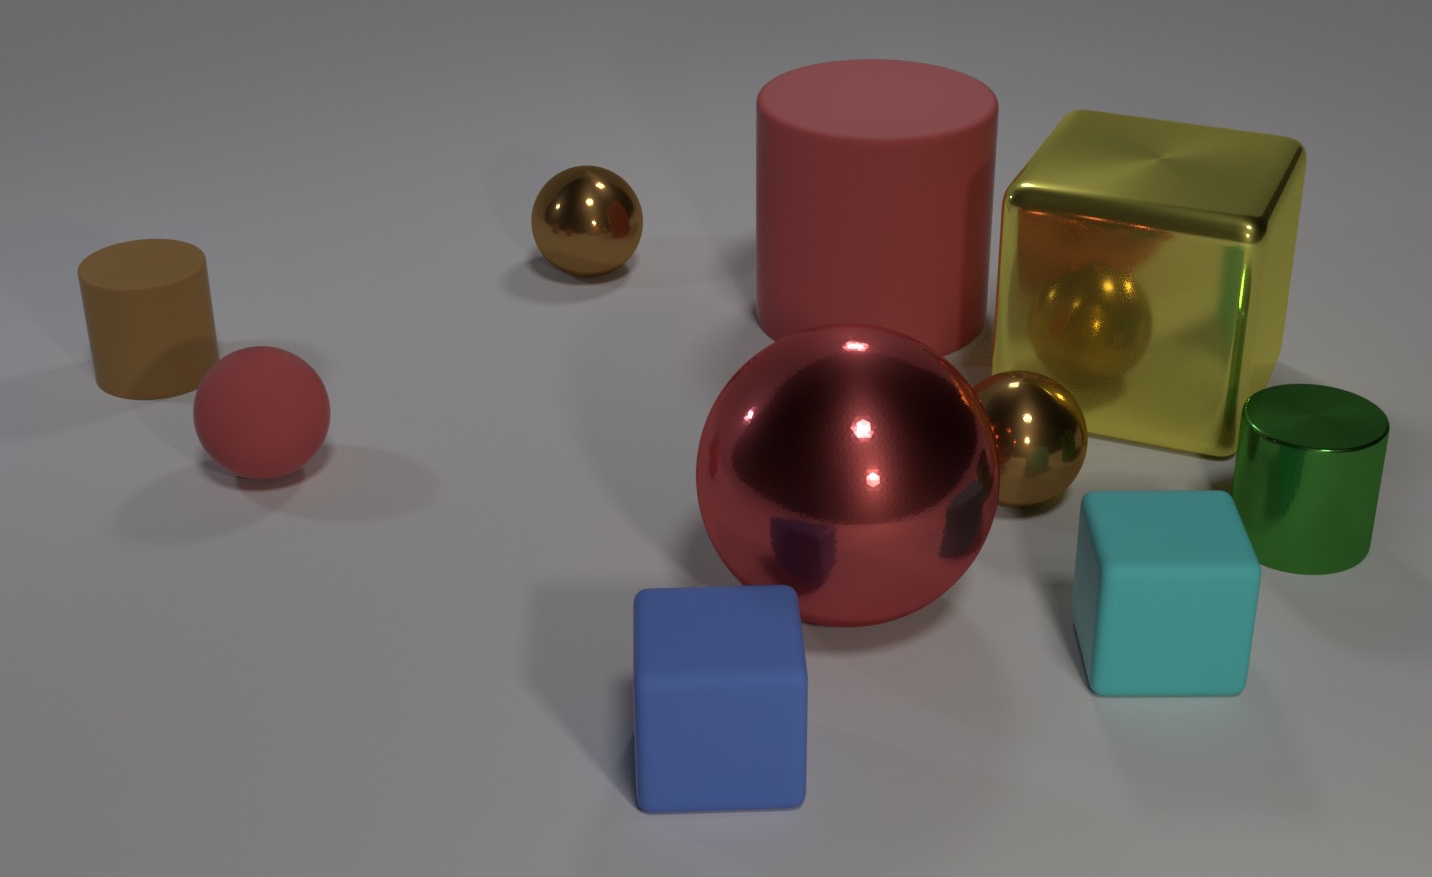
\includegraphics[width=.95\linewidth]{ch-dataset-task-benchmark/figures/dataset/original_clevr_image.png}
\caption{Original CLEVR image.}
\label{fig:dataset-clevr-image}
\end{spacing}
% \vspace{-.25in}
\end{wrapfigure}

CLEVR stands for Compositional Language and Elementary Visual Reasoning, aiming to provide researchers with synthetic (computer-generated) image dataset which allows asking different sorts of reasoning questions: comparisons, relationships, counting queries, etc. Each image in CLEVR is comprised of a number (usually 5-10) of objects, each defined by its shape (sphere, cube, or cylinder), color (one of eight options), material (metal or rubber), and size (small or large). After generating images, the CLEVR authors create queries for each image, each query an instantiation of a template filled based on the content of the image. A template such as \textit{"Do the \textless Z \textgreater \textless C \textgreater \textless M \textgreater \textless S \textgreater and the \textless Z2 \textgreater \textless C2 \textgreater \textless M2 \textgreater \textless S2 \textgreater have the same size?"} would allow asking a question such as \textit{“Do the red rubber sphere and the blue metallic sphere have the same shape?”} As these templates imply, the CLEVR database presents its queries in natural language (or as a functional program), challenging the models to reason over both textual inputs and images. Perhaps most importantly for our purposes, the authors made their entire codebase available on Github\footnote{\url{https://github.com/facebookresearch/clevr-dataset-gen/}} and did a rather reasonable job of documenting it. Their codebase uses Blender \parencite{BlenderOnlineCommunity2018}, a free and open-source 3D modeling software with a full Python API to generate the stimuli. Each stimulus is saved both as an image and as a JSON description of the scene, which allows generating valid queries and the correct answers for them. One additional source of inspiration was the Sort-of-CLEVR task introduced by \textcite{Santoro}. They provide substantially simplified visual stimuli (simple 2D drawings rather than 3D renders) and encode the questions as binary vectors, rather than natural language sentences. Sort-of-CLEVR also mixes both relational questions (\textit{``What is the shape of the object that is furthest from the gray object?’’}) and non-relational queries (\textit{``What is the shape of the gray object?’’}); the latter substantially more resembling the type of queries we decided to use.

\section{Dataset Generation}
The basic premise for our queries use is simple: we wish to train models to answer yes/no existence questions on an image. Using the original CLEVR image to the right as an example, we could query the model on \textit{``is there a purple object?''} (no), \textit{``is there a cube?''} (yes), \textit{``is there a red sphere?''} (yes), or \textit{``is there a cyan cylinder?''} (no). The CLEVR dataset is unbalanced, in that it includes eight colors, but only three types of objects (sphere, cube, and cylinder, all seen in the image above), and two materials (rubber and metal). To be able to examine the scaling behavior over the different tasks, and to avoid dataset-based biases for particular dimensions, we wanted to balance the image generation to have equal numbers of options in each dimension.

\begin{wrapfigure}{r}{0.5\linewidth}
\vspace{-.4in}
\begin{spacing}{1.0}
\centering
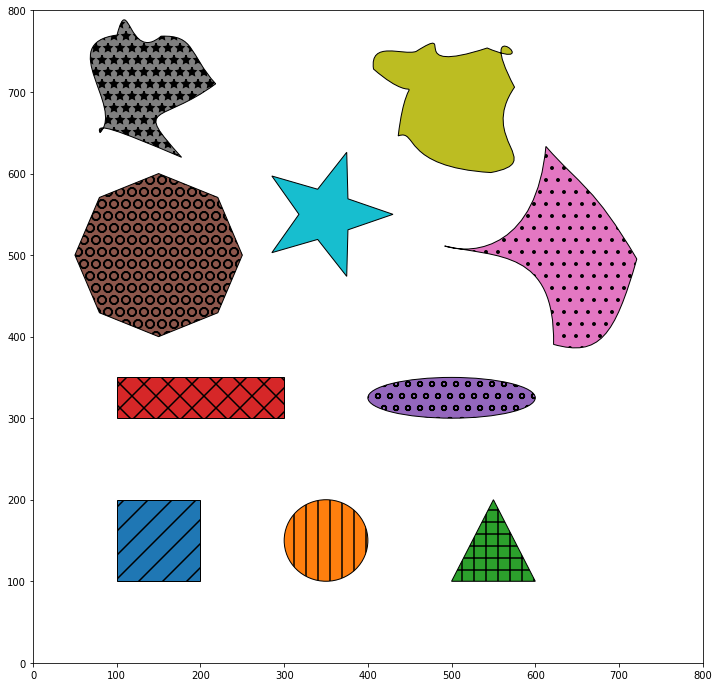
\includegraphics[width=.95\linewidth]{ch-dataset-task-benchmark/figures/dataset/matplotlib_image.png}
\caption{Matplotlib example image.}
\label{fig:dataset-matplotlib-image}
\end{spacing}
% \vspace{-.25in}
\end{wrapfigure}

We first prototyped examples using Python’s matplotlib \parencite{Hunter2007} to generate simpler stimuli (see example) but decided the results would be substantially more meaningful with a realistic visual task. We then set about adapting the codebase provided by \textcite{Johnson2017} to fit our purposes. We settled on ten colors, ten shapes, and ten materials, which provide thirty different single-property queries and three-hundred unique two-property (conjunctive) queries. 

\begin{wrapfigure}{r}{0.5\linewidth}
\vspace{-.4in}
\begin{spacing}{1.0}
\centering
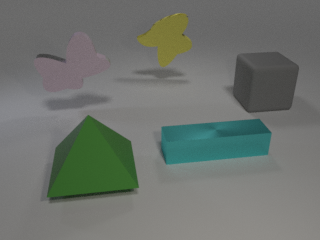
\includegraphics[width=.95\linewidth]{ch-dataset-task-benchmark/figures/dataset/first_iteration_image.png}
\caption{Example early iteration image.}
\label{fig:dataset-early-image}
\end{spacing}
% \vspace{-.25in}
\end{wrapfigure}

Choosing ten colors was easy: we picked ten reasonably equally perceptible ones\footnote{Gray, red, blue, green, brown, purple, cyan, yellow, orange, pink.} (or so we thought; we eventually discovered that our models have a hard time separating two of them). Next came the shapes: we initially created seven geometric shapes, relying on Blender’s built-in objects (such as a torus and a cone), but then realized we need additional shapes. We first experimented with different curve-enclosed shapes (in the background in the example to the right), but we were concerned with the stark difference between geometric shapes and the curved ones. After some creative thinking, we eventually settled on ten geometric shapes\footnote{Cube, sphere, cylinder, pyramid, cone, torus, rectangular box, ellipsoid, octahedron, dodecahedron}, from the mundane (cube, sphere), to elongations thereof (rectangular box, ellipsoid), to the more exotic (octahedron, dodecahedron). The materials proved the most difficult: the two in the original paper mostly differed in their reflectivity of incoming light. After following a myriad of tutorials, we realized the easiest path is to learn sufficient Blender skills to allow building image-based material textures. These allow transforming an image of a texture (e.g., bathroom tiles), alongside with maps describing the relative height at each pixel (allowing the creases between tiles to appear lower) and the reflectivity of each pixel to a Blender material definition. To apply these definitions, we also had to generate mappings from the three-dimensional surfaces of the objects to a 2D plane, on which Blender would overlay the textures; effectively, define how the objects should be cut and the surfaces laid flat. After passing through this myriad of obstacles, we were finally able to generate about fifteen textures, from which we selected ten\footnote{Metal, rubber, chainmail, marble, maze, metal weave, polka dots, rug, bathroom tiles, wooden planks.}, including the original rubber and metal, but ones as creative as a chain mail, a rug, or the previously mentioned bathroom tiles. 

\begin{wrapfigure}{r}{0.5\linewidth}
\vspace{-.2in}
\begin{spacing}{1.0}
\centering
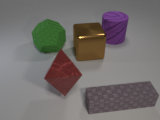
\includegraphics[width=.95\linewidth]{ch-dataset-task-benchmark/figures/dataset/final_image.png}
\caption{Example final iteration image.}
\label{fig:dataset-final-image}
\end{spacing}
% \vspace{-.25in}
\end{wrapfigure}

The image to the right is an example from the final dataset. Can you classify the shape, color, and material of each object?\footnote{Red marble octahedron, pink metallic weave rectangular box, brown metal cube, purple wooden plank cylinder, and a green chainmail dodecahedron.}

If you could tell shapes apart but had a hard time naming each color or texture, you could probably do sufficiently well, as the model is not tasked with learning the natural language mappings for these queries either. We introduce the questions to the model in binary encoding, similarly to Sort-of-CLEVR, as we wish to isolate the computer vision and meta-learning parts of the task from the natural language processing component. The query is provided as a 1x30 vector, with each block of ten units corresponding to a dimension (shape, color, and material), and each unit within a particular feature. The first unit might be mean `cube,' the twelfth `red,' and the twenty-fifth `marble.' A priori, the models will not know what feature each unit corresponds to, nor that each group of ten refer to a different dimension - but hopefully, effective meta-learning approaches will be able to extrapolate efficiently from their training, rather than pay the same cost (in training examples) for each new feature learned.  

While we made the task harder by including additional properties in each dimension, we decided to reduce a few other sources of variance, in an attempt to focus on the meta-learning. The original CLEVR dataset includes two different object sizes, while we only have one. They also include jitter, both in the orientation of the objects relative to the camera and in the precise location of the camera relative to the scene. We chose to keep both constant for now, reasoning that we could always generate a second dataset with additional visual noise should the task prove too easy. Each image we generate has four or five objects, each with a unique shape, color, and material. We settled on a size of 160x120 pixels, maintaining CLEVR’s standard 4:3 aspect ratio, but reducing each dimension by half, hopefully making the problem more computationally tractable. We also kept CLEVR’s method of assigning objects to locations in the scene randomly and checking for collisions, as it produced better results than two alternatives we examined, placing objects uniformly on a circle or in random locations on a 4x4 grid (both with some random noise to the assigned locations). The flexible nature of our implementation would allow us (or anyone else, once we make the code available on Github) to generate additional images using different parameters.

Once we settled on these final parameters for our dataset, we generated a total of fifty thousand images, split into a training set (45,000) and a test set (5000). See example images and corresponding scene descriptions (see below) here: \url{http://bit.ly/metalearning_50k_examples}. To generate these images, we used five virtual machines (VM) on Amazon Web Services (AWS). AWS offered easy access to machines with GPUs, which speed up the rendering process considerably, from about a minute per image to a few seconds, such that each VM rendered ten thousand images in just under a day. It could likely be optimized, as the object placement and collision resolution took more time (on average) than the scene rendering. We could have considered a more physically-based method, assuming each object repels other ones and simulating the dynamics between them; but the random placement proved sufficient for our purposes. We also did not attempt to explicitly balance the number of times each of the materials, colors, and shapes appear in the final dataset, and instead, we sampled them uniformly and trusted the sufficiently large sample size to overrule random fluctuations. While this worked successfully for most categories, about a month after generating the dataset we discovered some imbalances. Given 45,000 images (in the training set), four or five objects per image, and ten features within each dimension, we would expect each feature to appear, on average, in 20,250 images. The pyramid and the octahedron appear in approximately 12,000 and 14,700 samples respectively. We do not currently understand the cause, but we hypothesize that for some reason, the random placement struggled with those two shapes. If true, this underscores the need for a better placement algorithm than random assignments (or otherwise, for a better random number generator). 

Alongside each image, the script saved JSON file describing the scene. This description allowed CLEVR to parameterize their queries, knowing what sort of relational (and non-relational) queries should produce valid queries for this image. Since our queries are more straightforward than their ones, our process is equally simpler. Initial versions computed the answer for every one-dimensional query, saving a 30x30 matrix of queries (each row using a one-hot encoding), and a 30x1 vector of results (does that feature exist in the image). As this format would make designing the conjunctive queries harder, we then switched to saving a small table of object representations, which is 3x5 (dimensions x maximum number of items). In the event only four items are in the image, the last row is left empty. 

One last modification made is to provide an HDF5 file \parencite{TheHDFGroup1997} with all images and scene descriptions. Creating this file spared us from uploading fifty thousand files (or a RAR archive containing them), and was recommended in some places as an easy way to provide and package a dataset. While some recent opinions suggest against HDF5 (see \cite{Rossant2016}), we found it sufficient for our purposes, as it allows us to transfer the entire dataset in a single file.

\section{Overall Task Description}
We can consider each of the queries to be a logistic regression problem from image space to a binary answer (as all questions we currently train on are yes or no questions), and thus the meta-learning aspect comes in examining how much previously acquired queries help reduce the amount of training required to learn subsequent queries. The closest parallel in the literature is the visual question answering (VQA; \cite{Antol2015}) paradigm. Our task offers a different focus than those two existing ones: VQA primarily investigates integrating natural language understanding with visual reasoning, and CLEVR offers more uniform images and a smaller range of queries but challenges relational reasoning between objects. Our task modifies the stimuli, simplifying some aspects (visual noise, number of objects) and complicating others (number of colors, shapes, and materials) and removes the language component to allow focusing on meta-learning algorithms’ scaling performance. As currently formulated, this task also differs from other supervised computer vision problems: image classification requires assigning a single label to an object, and multilabel classification does not usually involve an explicit query. Semantic segmentation (labeling each pixel as part of an object) is a much harder visual task, with a substantially different output (a pixel map segmenting the image), and image captioning requires reasoning over similar visual information, but again, excluding a query and expecting a different form of output (a textual description).

Note that this task structure by itself does not necessarily investigate meta-learning. However, the structure of the task and dataset are crucial to the design of the two benchmark paradigms we propose, which do allow evaluating meta-learning capabilities:

\section{The Sequential Benchmark}
In this benchmark, we examine if and how much a model learns how to generalize between queries in the same dimension. Does learning to answer a few color-related questions help learn the next color related task more efficiently? To test this, we sequentially expose the model to tasks in a single dimension. In the first episode, we begin with a single task (\textit{`Is there a red object?'}), and train the model on it until it reaches criterion (95\% accuracy on the held-out test set). In the second episode, we add a second task to the training set (\textit{`is there a blue object?'}), retaining the first task in the training set (rather than continuing training only on the new one), in order to avoid catastrophic forgetting, and resume training and testing until reaching criterion on the test set in both tasks. If we do not set the criterion to be on both tasks, the model quickly forgets earlier tasks, as Figure \ref{fig:old-sequential-benchmark} demonstrates. We continue to mix in a new task in every episode in such a fashion, examining the time required to train each additional task to reach the threshold criterion. We wish to examine the amount of training (in total iterations performed) required to achieve criterion in each additional task, which would ideally asymptote toward some minimum, varying by the model architecture examined. We currently transition to the next task based on the held-out test set accuracy, but we realized in retrospect that it would be sensible to introduce a validation set for that purpose. Theoretically, by transitioning based on the test set, we allow it to influence the progress on the benchmark, and it would be preferable to do that based on a validation set and maintain an independent test set. However, since we do not allow the model to learn on these examples, and do not use them for hyperparameter selection, this should not raise an issue, since the same generative process would create the validation and test sets. We will consider introducing it should we revisit this benchmark in the future.  
\begin{figure}[!htb]
% \vspace{-0.225in}
\centering
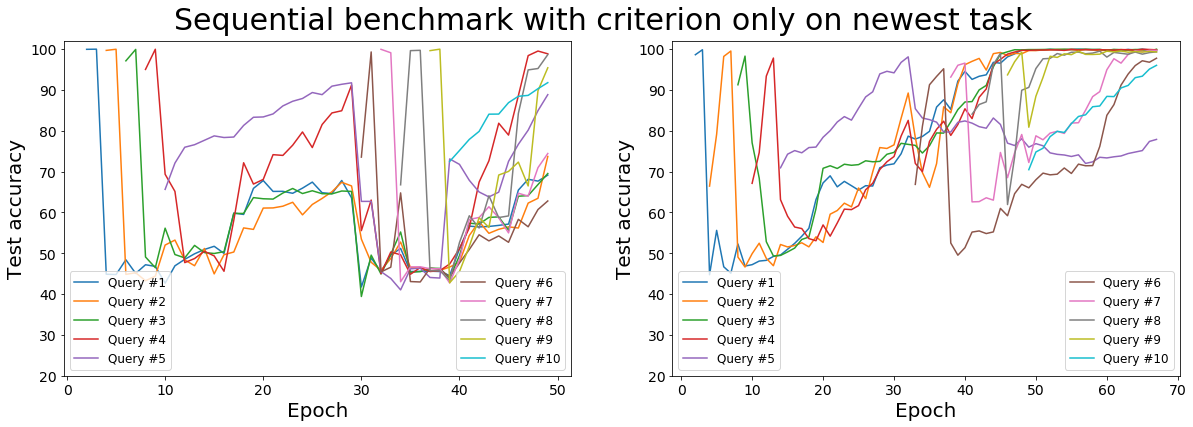
\includegraphics[width=\linewidth]{ch-dataset-task-benchmark/figures/benchmark/old_benchmark.png}
\caption[Sequential benchmark with criterion only on newest task.]{{\bf Sequential benchmark with criterion only on newest task.} The results of two example sequential benchmark iterations (using slightly different coreset settings and different random seeds) with the accuracy criterion only on the newest task. While in the right-hand side plot most query accuracies eventually improve, in the left-hand side plot many tasks fail to reach criterion. These results motivated setting the accuracy criterion to all tasks, rather than only the more recent task.}
\label{fig:old-sequential-benchmark}
% \vspace{-0.2in}
\end{figure}

To focus on the current task while maintaining previous tasks, we modify the coreset approach described by \textcite{Nguyen2018}. In every epoch, we assign a single query to each of the 45,000 training set images. We assign one half of the training set (22,500 images) to the current task learned, and the remaining 22,500, the coreset, are split as evenly as possible between the previously trained queries. On every epoch, we sample a new appropriately sized coreset for each previous task. We require the coreset not to be extremely imbalanced: if the ratio of positive to negative examples (in either way) is more than 4:1, or in other words, if either positive or negative examples reflect under 20\% of the coreset for a given task, we sample it again. After sampling the coreset, we assign the remaining 22,500 images to the current task and begin training. 

Note that as we acquire additional previous tasks, each one receives fewer coreset examples in every epoch. The diminishing repetition of past tasks could also be viewed as a sort of distributed practice, which relies on the spacing effect, as a method of improving memory recall (cf. \cite{Bahrick1993}; \cite{Russo1998}). We treat the test set in a more standard fashion, evaluating each of the 5000 test set images using all active (current and previous) queries.

To avoid sensitivity to the order in which we introduce the tasks, we average this scaling behavior over several different executions, each execution adding the tasks in a different order. To further mitigate the potential for order-related effects, we employ a Latin square design (see \cite[][ch. 9]{Bailey2008}), which guarantees that for each ten-replication block, each task will appear in each ordinal position (first, second, and so on) exactly once. We do not currently account for second-order effects (how often a task appears before or after another task). To generate these designs, we take a standardized Latin square (which has the first row and column both perfectly ordered), permute the rows once and columns once, and take the appropriate row for the index within the current ten-replication block \parencite{InteractiveStatisticalPages}. When comparing different models, we will use the same random seed for the row and column permutation, guaranteed we compare on identical column orderings. 

We currently investigate each dimension independently, examining different orderings of the colors, shapes, and materials. There is a stronger shared structure when training only within a single dimension, which should make the meta-learning problem easier. We also developed a control condition, which attempts to examine how the degree of shared structure between the tasks helps accelerate training. Rather than train on all ten tasks from a single dimension, we train on random sets of ten tasks across all three dimensions. To control for the order of introduction between the dimensions, we cycle through the six permutations of dimension orderings\footnote{Color-shape-texture, color-texture-shape, shape-color-texture, shape-texture-color, texture-color-shape, texture-shape-color.}, sampling a task from each dimension until we reach a set of ten. We then train on these ten tasks following the benchmark protocol outlined in this section. If the model learns to exploit shared structure within a dimension, it might be slower in this condition than in the single-dimension condition, since the model has a lower degree of shared structure to exploit between the tasks. However, if the model shows benefits from overall improved visual processing, this condition might not be more difficult, and in fact, might elicit lower interference between the tasks learned.

This task allows us to explicitly evaluate how learning scales as a function of the number of previously learned related tasks. We can measure how many training examples does it take to learn a task for the first time, as a function of how many tasks have been previously learned. We can also measure how many examples it takes to re-learn a task, to overcome the interference introduced by adding a new task, as a function of the number of times the task has already been relearned. We can also quantify the catastrophic interference induced by adding additional tasks, both as a factor of how many tasks the model already knows and as a factor of how many times the model was trained on a particular task. The benchmark we describe is not unlike the incremental learning setting suggested by \textcite{Kemker2017a}, although our coreset of previous task examples aids models in retaining previous tasks, which the authors there do not afford, making their setting more challenging.

A note regarding terminology: we borrow the term \emph{episode} from the meta-learning literature, and use it to refer to each stage in the benchmark with a fixed number of tasks. In other words, the benchmark is comprised of ten episodes, the first with one task, and the second two, and the last with ten. Each episode requires one or more \emph{epochs} to complete, where an epoch is one pass through the entire training set, with each training example allocated to a single active task. 

\section{The Compositional Benchmark}
The description of this benchmark will be less detailed than the previous one since this is a second benchmark we foresee implementing with this dataset and task structure but have not implemented yet. We describe it to demonstrate additional investigations this dataset and task structure would allow us to pursue: 

In this benchmark, we will examine a different sort of meta-learning: if a model learns two parts of a composite query, does it make it easy (or ideally, immediate) to learn composite queries as well? We can consider several different phases of this benchmark: in the first, we train a model on several single-item tasks (``Is there a red object?'' ``Is there a torus'') until reaching criterion. Once the model performs adequately on these tasks, we begin training on composite tasks (``Is there a red torus?''), composed entirely from tasks the model reached criterion on, monitoring how much additional training is required to achieve criterion on these conjunctive tasks from previously-trained single-item queries. 

In the second phase, we introduce additional features in each dimension without training on them individually. We now train on composite queries involving one previously trained feature and one new one (\textit{`Is there a red pyramid?’ `Is there a teal torus?’}), again training until reaching an accuracy threshold on all such queries. In the final training phase, we introduce the remaining colors, materials, and textures, and examine how much additional training is required for learning their conjunctive queries. As in the previous phase, we do not train on the single-item queries. The training is complete once the model reaches the accuracy criterion on all two-item conditions. 

To evaluate the quality of representations learned, and go beyond the number of iterations required to finish the benchmark, we can evaluate the models on all single-item queries. As this benchmark is currently formulated, we train the models on the single-item queries only on the features introduced in the first phase. If a model learns to exploit the shared structure between items, it should fare well on the individual queries as well. Performing this additional test would allow us to not only quantify the scaling behavior as a function of compositionality but additionally the robustness and quality of representations learned. 

As with the previous benchmark, we would randomize the order in which tasks are introduced to the model, employing a similar Latin square design to the previous benchmark. The task order implies which features/tasks are trained on individually, and which ones are only introduced as part of the composite tasks. We would average over different such random training subsets to evaluate each model, but make sure to evaluate all models on the same task orderings, to make sure the comparison is valid. 

% 
\chapter{Models Compared\label{ch:models-compared}}
All models compared in this work were implemented in PyTorch \parencite{Paszke2017}.
\section{Baseline Model}
This model is inspired by the CNN+MLP model used by \textcite{Santoro} on their Sort-of-CLEVR dataset and modified in resemblance to the VGG-16 architecture introduced by \textcite{Simonyan2014}. The overall architecture of this model includes a convolutional neural network (CNN) which extracts features from the input image, followed by a fully connected network (also referred to as a multilayer perceptron, or MLP) which processes the extracted features and query into an answer (\textit{`Is there a red object?' $\to$  `yes'}). 

A convolutional neural network (CNN) is a neural network architecture often used in computer vision problems, or other domains where the input has a spatial structure where we expect some degree of spatial invariance -- in our task, a sphere should be recognized as a sphere regardless of where in the image it appears. Each layer group in our CNN begins with the convolutional layer, which applies a set of filters at every location in the image (the convolution operation). After each filter computes a value at every location, the layer group continues with a nonlinearity function, batch normalization (in order to account for differences between batches), and local pooling (in order to reduce the spatial dimensions between layer groups). The specific architecture employed in this model includes four layer groups, with 16, 32, 48, and 64 filters in each one. Each filter is 3x3 units, moved with a stride of 1 and padding of 1, and the pooling units reduce each 2x2 unit block to a single unit - halving the input size between layers, or doubling the effective receptive field of units between layers. The output of the last convolutional layer group has dimensions 64 (filters) x 10 (width) x 7 (height). 

To feed the convolutional output to the next, fully connected layer, we need to flatten it, as fully connected layers receive a vector as their input. We, therefore, flatten the output above to a $64 \times 10 \times 7 = 4480$ unit vector, to which we concatenate the 30-unit query representation, arriving at a 4510-unit input to the fully connected network. The fully connected network has four such layers, each with 512 hidden units, also using the ReLU activation function, before the final layer, which has two units. We interpret these units as the probability assigned to `yes' and the probability assigned to `no’ on our binary queries. We used the cross-entropy loss function, which evaluates the model based on how much of the probability mass the model assigned to the correct answer. 

The following schematic describes the model: the initial blocks are the convolutional ones, where the layers retaining spatial size and increase depth are the convolutions, and the layers maintaining depth and reducing size are the pooling ones. The eventual representation is flattened, the query is appended to it, and it is then passed to the fully connected layers.
\begin{figure}[!htb]
% \vspace{-0.225in}
\centering
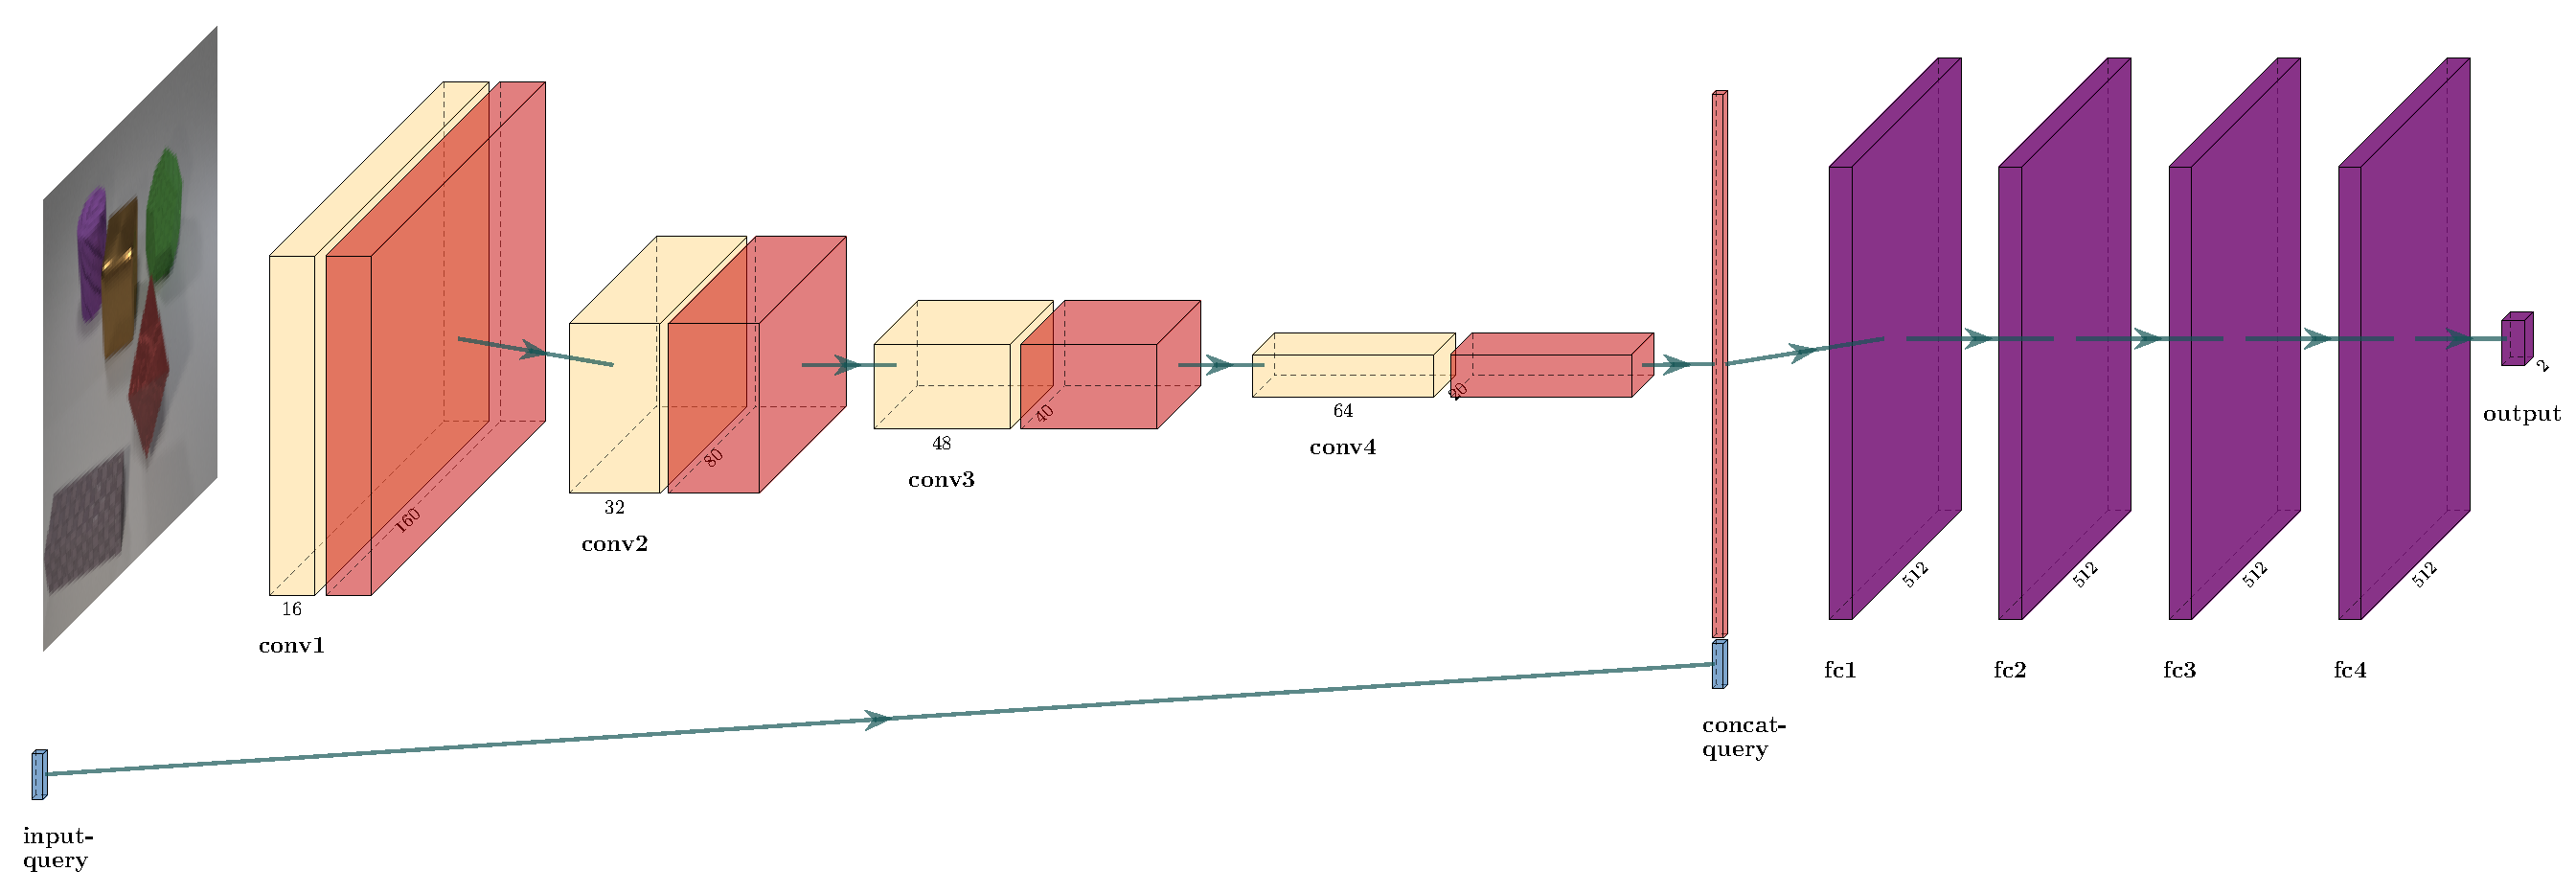
\includegraphics[width=\linewidth]{ch-models-compared/figures/baseline.pdf}
\caption[Baseline model diagram.]{{\bf Baseline model diagram.} The model is presented with an input image, which is passed through four convolutional layers groups, each including a convolutional layer, non-linearity (ReLU), batch-normalization and 2x2 max-pooling. After the fourth convolutional layer group, the representation is flattened to a vector and concatenated to the input query. The concatenated representation is then passed through four fully connected layers, before a final output layer with two units. \emph{Yellow layers:} convolutional layers, \emph{orange:} max-pooling, \emph{purple:} fully-connected, \emph{blue:} the input query.}
\label{fig:baseline-model-diagram}
% \vspace{-0.2in}
\end{figure}

Initial experiments on the entire dataset, presenting all thirty single-feature tasks together, demonstrated that the model was overfitting the training set, as at some point through training, the test-set accuracy and loss stagnated, while the loss on the training set continued dropping, and correspondingly, the training set accuracy continued rising. We then experimented with several measures designed to prevent overfitting. Dropout is one such measure, which during training randomly turns off random units in each layer, intuitively forcing the network to learn to build in some redundancy to how it solves the task, therefore improving its robustness. We experimented with both forms of dropout, standard \parencite{Srivastava2014} for the fully-connected layer, and spatial dropout \parencite{Tompson2015}, which turns off entire filters (again, encouraging redundancy between them) in convolutional part of the network. Another measure we attempted is weight decay \parencite{Krogh1992}, which puts a small penalty on the magnitude of the weights, encouraging weights to remain smaller (and corresponding to a zero-mean Gaussian prior on the weights). We also introduced a learning rate scheduler, to reduce the learning rate when the network gets ``stuck,'' allowing it to perform granular tuning at that point. Of these, weight decay proved by far the most effective (see results below), the learning rate scheduler only helped with minor tuning, and dropout proved ineffective. Therefore, we perform the sequential benchmark experiments reported below with weight decay (using a penalty of 1e-4) and without the learning rate scheduler or dropout. All models were fit using the Adam \parencite{Kingma2015} optimizer.
\section{Query-Modulated Visual Processing Model}

Most models for tasks that resemble ours, such as VQA \parencite{Antol2015,Agrawal2016}, CLEVR \parencite{Johnson2017}  or Sort-of-CLEVR \parencite{Santoro}, tend to follow a similar form to the baseline model described above. First, we pass the image through a convolutional neural network, which processes it into some embedding (or latent representation) which the model can reason over. If the query is provided in natural language (as it is in VQA or CLEVR), it is independently processed to a separate embedding, almost always using a recurrent neural network. We then combine these two embeddings, of the question and of the image, and present the combined representation to another neural network, which attempts to compute the answer to the question on the image. A variety of different architectures have been proposed for these tasks, all broadly matching this description. These include several models examined by \textcite{Antol2015} in their work presenting the VQA paradigm, most models presented by \cite{Johnson2017} when introducing CLEVR, and the relational neural network discussed in \textcite{Santoro}. Several alternative models for these tasks propose defining and learning a set of individual ``modules,'' such ones to find particular objects or filter them based on relations, and learn both the weights for these modules as well as how to combine these modules to answer each query, building a unique computational graph for each different type of query \parencite{Johnson,Hu2017}. These models are substantially more powerful but correspondingly harder to implement and substantially more challenging to train.
\begin{figure}[!htb]
% \vspace{-0.225in}
\centering
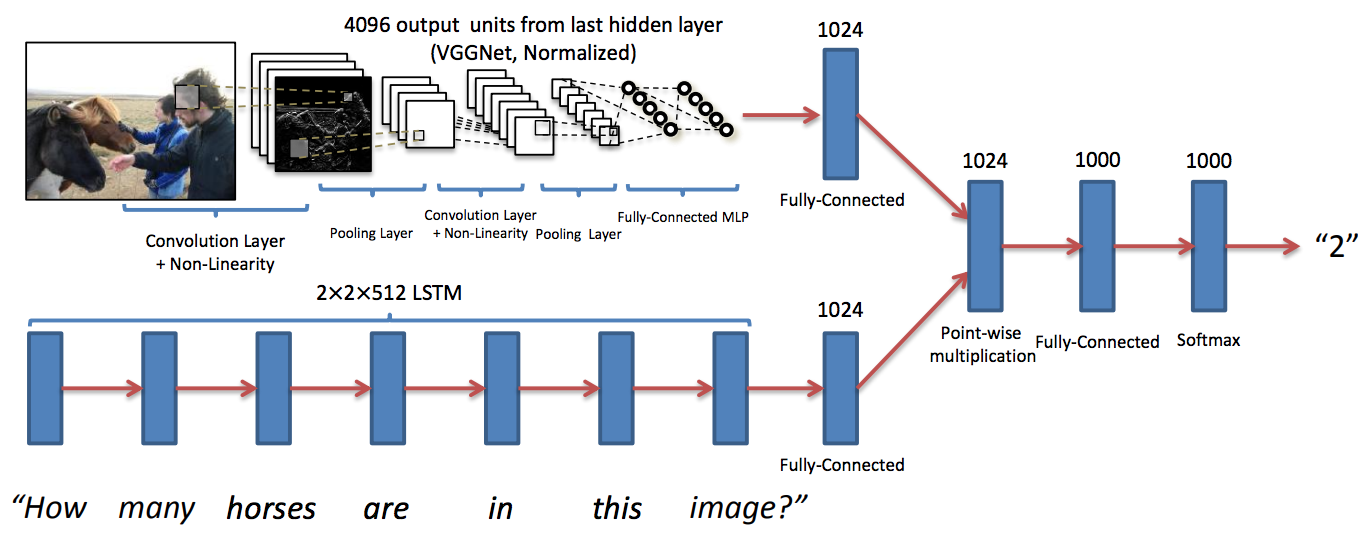
\includegraphics[width=\linewidth]{ch-models-compared/figures/reproduced.png}
\caption{{\bf VQA model diagram.} A schematic describing \possessivecite{Agrawal2016}'s best model, which independently processes the image and the question, combined the embeddings using element-wise multiplication, and feeds the combined embedding to a fully-conencted network to produce an answer. Reproduced from \textcite{Agrawal2016}.}
\label{fig:vqa-model-diagram}
% \vspace{-0.2in}
\end{figure}

We propose a model that strikes a middle ground between the two approaches described above, inspired by \textcite{Mozer2008}. In the first set of approaches, the image is processed into an embedding entirely independent of the query, which means that if we attempt to answer two separate questions on the same image, we will use the same visual embedding, only differing in the final, combined processing stage. On the other hand, we hoped to arrive at a model which does require the tremendous flexibility (and hence, complexity) of computing a different computational graph for each query. We found inspiration in the human visual system, where there is evidence for a tuning or modulation effect based on the task performed. \textcite{Cukur2013} use functional imaging to demonstrate that when subjects are asked to search movies for particular categories, such as `humans' or `vehicles,' their semantic representations shift to prioritize these categories, even when they do not exist in the stimuli presented. \textcite{Kay2015} and \textcite{Bracci2017} provide additional evidence for task-based and attentional modulation, impacting both the effectiveness of spatial coding and which properties of objects are represented. There is substantial recent research on how convolutional neural networks, on which our model is based, not only solve tasks well but also model activity in the human visual stream accurately \parencite{Yamins2016}. This line of work has produced a number of modifications to convolutional neural network architectures, which seek to augment these artificial models with additional features of the human visual system, such as recurrent and feedback connections \parencite{Spoerer2017,Nayebi2018} or different convolutional layers \parencite{Kubilius2018}. 

We offer a relatively uncomplicated approach which introduces the minimal augmentation to the baseline architecture that would enable query-based modulation. Recall that in the baseline model, the four convolutional layer groups included 16, 32, 48, and 64 filters respectively. In a convolutional architecture, each of these filters is passed over every spatial location in the input to that layer, computing a value for each location, which is then passed through an activation function (ReLU), batch-normalized, and pooled with adjacent values to be passed onto the next layer. To allow for query-based modulation, we introduce an additional layer, which maps from the query (a 30x1 vector) to the filters of a particular convolutional layer. The intuition is that different filters might be differentially relevant to distinguishing different properties of the input, and therefore being able to amplify or dampen the output of specific filters based on the query will help the model perform the task more effectively. This formulation allows us to achieve query-based modulation at miniscule additional computational cost, requiring only a single additional layer with under 2000 new parameters\footnote{The input (the query) is 30 units, and a bias unit is usually added. The maximal output size is 64, the number of filters in the last layers. Therefore, this layer requires $(30 + 1) \times 16 = 496$ weights to modulate the first convolutional layer, and $(30 + 1) \times 64 = 1984$ weights to modulate the last one.}. We compared each of the four possible depths of modulation, of augmenting each of the convolutional layer groups, as we did not know a priori which one (if at all) might produce results. Our approach is more naive than other modulation-based approaches, such as GaterNet \parencite{Chen}, who employ a secondary network to elect which filters to gate from a primary one, or FiLM \parencite{Perez2017,Dumoulin2018}, who employ a more complicated model architecture and interpret the modulation as conditioned normalization, an extension of batch normalization which normalizes based on the current input.   

In the context of our task and the sequential benchmark, we wish to examine a few questions. First, does introducing such query-based modulation improve the capacity to learn the baseline task (simultaneous, heterogeneous dimensions) -- that is, if we train a model on all thirty single-feature queries, using task-based modulation after the first, second, third, or fourth convolutional layer group, would it be able to learn the task faster. Second, if it improves performance with the entire dataset, will it behave similarly on the sequential benchmark? In other words, does it improve the capacity of the model to learn all queries simultaneously, or does it also improve the capacity to acquire the queries one at a time? Third, if it does improve performance on the sequential benchmark, does it demonstrate better scaling behavior? To elaborate this question, let us assume a query-modulated model indeed learns the queries faster when introduces in the sequential benchmark. Is it learning the initial queries more rapidly, but achieving similar performance on later ones? Is it learning all queries faster, but early queries equally faster as later ones? Alternatively, is it improving the scaling behavior, increasing the advantage over the baseline model as additional queries are introduced?


\chapter{Results\label{ch:results}}

\section{Baseline Model Capacity (Simultaneous, Heterogeneous Dimensions)}
Before beginning to evaluate this model on the sequential benchmark described above, we wanted to verify it has the capacity to learn our intended task in a non-meta-learning context. We trained different variants of the model described above on the entire training set, evaluating the model on all single-item queries on every image on the test set after each epoch. We reasoned that in order to merit investigating meta-learning using this model, we should first prove it has the capacity to solve these tasks in an easier setting. We term this condition as simultaneous (rather than sequential), heterogeneous dimensions (using queries from all three dimensions, rather than homogeneous conditions, which use queries from a single dimension).

The initial dataset we generated included 4096 stimuli (split 7/8'ths training and 1/8'th test), using eleven shapes and ten colors, and without querying on materials, since at the time we only had two of them (the two we inherited from CLEVR). The model as described above failed to learn the task well and overfit the training set. An example overfit execution from an early run demonstrates a plateau in the test set loss (left) and accuracy (right), while the performance on the training set continues to improve:  

\begin{figure}[!htb]
% \vspace{-0.225in}
\centering
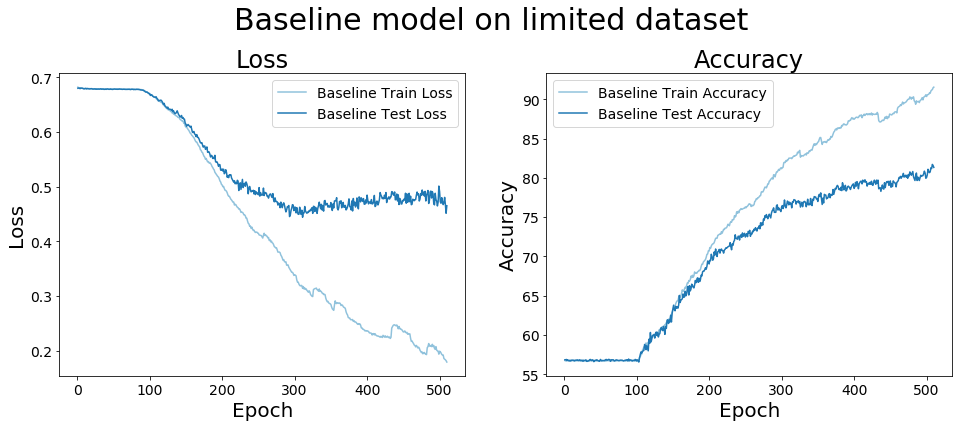
\includegraphics[width=\linewidth]{ch-results/figures/baseline/limited_dataset.png}
\caption{{\bf Baseline model on initial dataset.} This model shows substantial overfitting }
\label{fig:results-baseline-limited-dataset}
% \vspace{-0.2in}
\end{figure}

These concerns were alleviated when we successfully generated the final, full dataset, which includes an order of magnitude more images (45,000 training, 5000 test), as well as the final collection of shapes, colors, and materials we intended to use. In an attempt to quantify performance better, we switched from accuracy to another measure, the AUC ROC (area under the receiver operating characteristic curve), which considered the performance of the model across different decision thresholds. Whereas the accuracy is computed with a fixed decision threshold between classifying as positive and negative, usually 0.5, the ROC score is computed by comparing the false-positive and true-positive range across all possible threshold values, from zero to one, providing a more holistic measure of the model’s success. The baseline model described above, without any measures to aid generalization and prevent overfitting, proved far more successful in learning the task on the full dataset, even if it did show some overfitting:

\begin{figure}[!htb]
% \vspace{-0.225in}
\centering
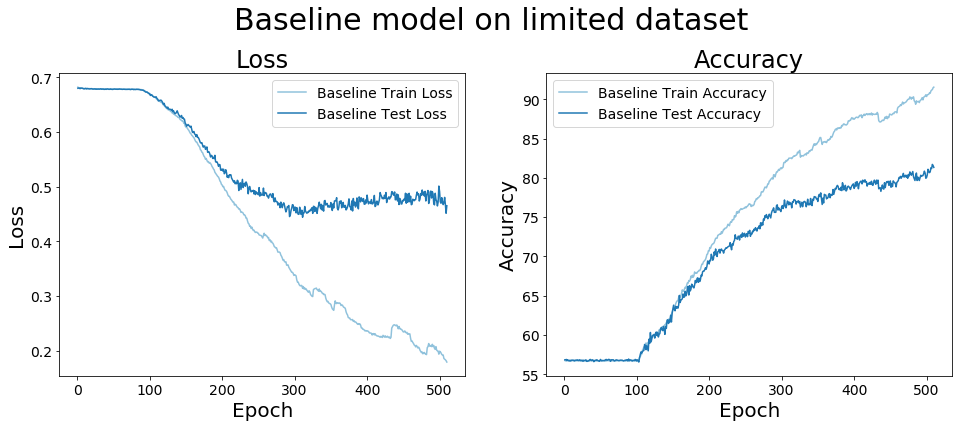
\includegraphics[width=\linewidth]{ch-results/figures/baseline/limited_dataset.png}
\caption{{\bf Baseline model on initial dataset.} }
\label{fig:results-baseline-limited-dataset}
% \vspace{-0.2in}
\end{figure}

In an attempt to alleviate the overfitting, we experimented with two fairly standard modifications, as outlined in the models compared section. Below are the results from adding dropout to the fully connected layers, and adding weight decay to the entire model. Both were added in tandem with allowing the learning rate to drop if the loss fails to improve for ten consecutive epochs. We were surprised to discover that despite the prevalence of dropout in the literature, it failed to learn well in this task; we might have investigated why, but having discovered that weight decay works spectacularly well, we opted to use it instead. Training with dropout, the loss peaks higher, the AUC does not reach 0.70, whereas training with weight decay goes about as ideally as one could imagine:

While there is still a minor discrepancy between the test and train losses, it is miniscule compared to previous results, and the test accuracy and AUC peak higher with weight decay than without (without: accuracy 95.63\%, AUC 0.9607; with: accuracy 98.69\%, AUC 0.9905). We therefore employ this model with weight decay in all experiments reported below.



\chapter{Conclusion and Discussion\label{ch:conclusion}}

We presented an original dataset and a visual question answering-inspired task design, which together allowed us to create one novel benchmark and suggest another one. The sequential benchmark we implemented allows examining how a model's learning performance changes with the number of tasks it already learned and with how many times it relearned each particular task. To measure how learning scales, we examined the number of examples a model required to learn a task to a 95\% accuracy criterion. To quantify catastrophic interference, we tested the accuracy immediately after introducing a new task to the model. We first examined how a baseline model, comprised of a simple convolutional neural network followed by a fully connected neural network, fared on this sequential benchmark. We then compared this baseline model to a set of models performing query-modulated convolutional processing, allowing the query to adjust the visual processing of the image presented, and analyze how performing this modulation at different layers of the convolutional model impacts performance.

We discovered that the baseline model, which is the minimal model we expected to be able to perform this task, shows positive scaling behavior: the more tasks it learns, the faster it tends to acquire the next task presented. This result was not intuitive to us -- we interpret it as suggesting that gradient-based optimization, coupled with this sequential presentation of tasks, allows the model to iteratively improve the quality of the weights it learns, putting it in a better starting position to acquire the next task. We consider this as an example of meta-learning, of learning how to improve the learning process for subsequent tasks. This result is different than previous models of gradient-based meta-learning, e.g., \textcite{Hochreiter2001}, which uses standard gradient descent to learn, but requires a recurrent neural network controller which functions as the meta-learning system. This work demonstrates meta-learning characteristics using a fairly naive model, with no specialized architecture. We note that model-agnostic meta-learning (MAML; \cite{Finn2017}) explicitly optimizes for weights that would be beneficial in learning multiple tasks, and we predict that an explicit meta-learning algorithm would perform better than our naive model. We find it intriguing that a model with no specific meta-learning features, neither in the architecture nor in the optimization procedure, demonstrates this type of positive scaling with additional training.

Conversely, when we examined the degree of catastrophic forgetting exhibited by this model, we discovered that the baseline model shows higher degrees of forgetting as it learns additional tasks. In the first episode introducing a new task, accuracy on the first few tasks the model learns dropped to around 75\%, while the accuracy on tasks introduced later falls to about 55\%. As noted above, the tasks introduced later also required fewer training examples to reach this criterion in first place. We interpret this behavior as an example of a stability-flexibility tradeoff (see \cite{Hermundstad2011}), in which over the course of the benchmark, the model acquires representations that are more flexible (and allow for faster learning) but are also less stable (and therefore show more rapid losses). It would be interesting to attempt to visualize these representations as a model learns additional tasks and see if we can find evidence for this stability-flexibility notion in the data. While tasks introduced later show higher forgetting, this effect tapers off after a task was trained on for a few times, showing a consistently lower degree of forgetting with additional training. In other words, what helps mitigate catastrophic interference is not domain expertise, which is acquired by learning additional tasks, but further practice with the same task. 

Our results on the control (sequential, heterogeneous dimensions) condition suggest that the interference for repeated learning within a dimension, on the baseline model, is higher than any benefits conferred by accruing knowledge within the domain of a particular dimension. An alternative interpretation might be that training on multiple dimensions, rather than a single one, encourages the model to retain additional types of visual information, which compete less, conferring an advantage rather than a disadvantage. The transfer occurring is therefore not dimension-specific, but rather a general improvement in the model's visual processing capacity. It is possible that if the heterogeneous tasks were more diverse, either including substantially different stimuli, or a variety of different computer vision paradigms (such as classification, semantic segmentation, and object detection), interference between tasks in the heterogeneous condition would be higher than in the homogeneous condition.

The query-modulated models show an improvement in some of the learning metrics examined, but not others. Query-modulation on all levels helps to learn the first few tasks faster and does not show the highly anomalous behavior in the second repetition of the first task, suggesting perhaps that the representations learned are stabler. However, both later times trained on the first few tasks, as well as all times trained on the tasks introduced later, show no such effect, and in some cases, the effect even reverses. This finding may imply that the representations the baseline, non-query modulated model acquires later in training are similar to the ones the query-modulated models learned from the beginning, another question we could investigate by visualizing the representations. While the query-modulated models all show the power law of practice effect on each task, as evidenced by the linear behavior in the log-log plot, they show weaker evidence of positive scaling within the domain for tasks introduced later. 

In catastrophic forgetting, the query-modulated models all do substantially better. All query-modulated models show higher accuracies in the first episodes introducing a new task, with the most robust effect in the second and third times the model learned each task, and for the earlier tasks a model learns. If we ascribe to the stability-flexibility tradeoff interpretation described above, query-modulation enables learning equally flexible representations that are more stable than those acquired without query-based modulation. In some sense, it is sensible that query-modulation of the visual processing should allow for this increased stability, as the model might achieve the required flexibility by changing the weights associated with the query, rather than with the convolutional filters; but we do not find these results obvious. 

The different performance profiles on the two aspects examined in this benchmark, the scaling behavior of the learning performance and the proclivity to catastrophic forgetting, reinforces the benefits of measuring and analyzing both. To paint a full picture of how well a particular model architecture or optimization procedure is capable of learning, we see demonstrable value in reporting how quickly a model learns new tasks, as a function of the number of previously acquired tasks.  Most existing meta-learning work ignores this framing, instead choosing to report the capacity to learn new tasks from a fixed small number of samples. We also believe that measuring forgetting should be an inherent component of making learning-related claims, as if a task is immediately forgotten when the model transitions to a new one, it weakens the notion it truly learned it before. 

We found the perspectives introduced by paralleling machine learning and human learning illuminating. Both the baseline model and all query-modulated models we examined show a power law of practice behavior in the number of examples required to reach criterion, as a function of the number of times the task was trained on. Human learners show robust evidence for such power laws, although usually examined in reaction time to response, rather than the additional practice required to maintain performance \parencite{Newell1980,Donner2015}. We provide an interpretation of some of the learning dynamics of the models as exemplifying the stability-flexibility tradeoff usually investigated in studies of memory, and believe it provides a useful perspective on these results. Our sequential benchmark maintains a coreset for practicing of previously learned tasks, which has a fixed size in every episode. The fixed total size with an increasing number of tasks results in fewer examples per episode for each previous task as the benchmark proceeds. This formulation could be considered analogous to spaced practice, in which as materials are learned better, they receive fewer repetitions \parencite{Spitzer1939,Greene2008}. From this perspective, allocating an equal number of examples to each previous task may be unideal, compared to assigning more practice to more recently-introduced tasks. To expand in this direction, we could investigate different coreset allocation methods, drawing more on the science of learning literature, and examine how these changes impact performance on the benchmarks. Ideas from cognitive psychology have been recently employed to help understand how neural networks function, with neural networks able to recover similar behavior to humans in a shape-bias test \parencite{Ritter2017} and in an experiment examining closure, recognizing objects as more than the sum of their parts \parencite{Kim2019}.
 % Conclusion
\section{Future Work}
We see several lines of work emanating from these results. We hope to take existing meta-learning and lifelong learning models and examine their performance on this benchmark, to measure the effectiveness of specialized architectures, compared to our baseline and query-modulated models. We are curious to see if any existing approaches confer benefits to both the scaling behavior and the degree of catastrophic forgetting, or if, as we might expect, approaches from the meta-learning literature aid in learning faster, while approaches from the lifelong learning field reduce the amount of catastrophic forgetting observed. We also plan to implement the second benchmark we described, which will allow us to investigate the scaling behavior of learning and the degree of forgetting exhibited in a compositional setting, which better mimics the demands of learning to reason in the real world. When we do that, we will use the lessons learned during the execution of the sequential benchmark. We are considering using a validation set to govern the transition between the phases of the benchmark, rather than determining when to introduce the next task based on the performance on the test set. We might also change one of the perceptually challenging colors, to remove that source of noise in the final results. If we modify the sequential benchmark, we might also investigate different coreset allocation schedules, drawing on the distributed practice literature in cognitive psychology.  

In the discussion, we outlined several interesting analyses we could perform by analyzing the representations learned by these models as they progress in the sequential benchmark. We posit several hypotheses for how the different models we benchmarked navigate the stability-flexibility tradeoff, and how representations might change over the course of training. While there is substantial literature on visualizing convolutional features through training \parencite{Zeiler2014,Olah2017}, we are unaware of any work visualizing features and representations in a meta-learning setting, and examining how representations shift as the model learns additional tasks. We could also attempt to visualize the effects of query-based modulation, which would allow to reason about which convolutional features contribute to the identification of which features. As with the dataset and benchmarks, which we will make available to the research community, we hope that developing novel ways to examine representations during the course of meta-learning will elucidate the behavior of these algorithms and drive research in this realm forward.

We also noted that our formulation of task-based processing is more straightforward than existing approaches, such as FiLM 
\parencite{Perez2017,Dumoulin2018}. Our results demonstrated that modulation at the later convolutional stages provided better results than earlier ones, but that may be conflated with the fact that introducing query-modulation at a later layer allows learning more parameters. This growth in the number of parameters is because our architecture includes more filters in each successive convolutional layer, which corresponds to the size of the query-modulation layer. We could perform ablation studies using models with equal numbers of filters in every convolutional layer group, and see if the effect holds. We are also considering investigating our simple query-based modulation in more complicated settings, such as CLEVR, or one of the visual question answering datasets. 
  % Future work


\appendix % all chapters following will be labeled as appendices

\chapter{Additional Figures\label{ch:additional-figures}}

\section{Query Modulated Models Capacity \label{sec:additional-figures-query-mod-simultaneous}}

\begin{figure}[!htb]
% \vspace{-0.225in}
\centering
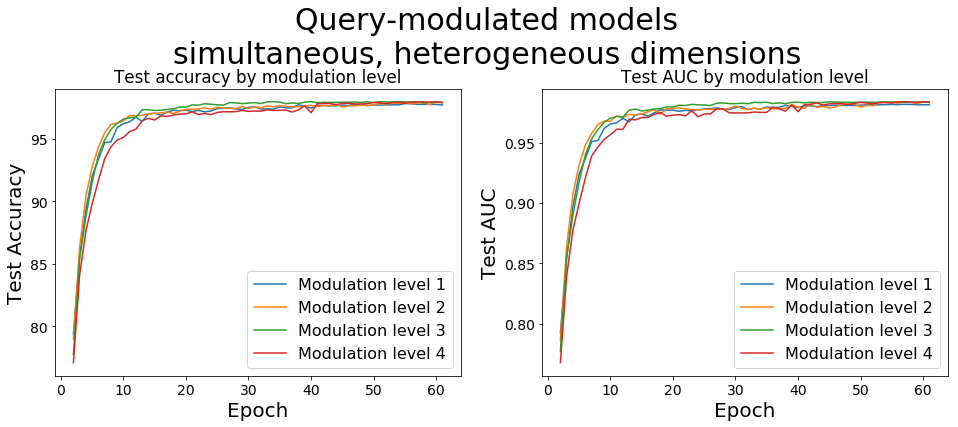
\includegraphics[width=\linewidth]{ch-results/figures/query_mod_simultaneous/query_mod_only.png}
\caption[Query-modulated models on simultaneous, heterogeneous dimensions.]{ {\bf Query-modulated models on simultaneous, heterogeneous dimensions.} This plot matches \ref{fig:results-query-mod-simultaneous-baseline-comparison}, but removes the baseline model, comparing only the four query-modulated ones. These models are still fairly inseparable.}
\label{fig:results-query-mod-simultaneous-query-mod-only}
% \vspace{-0.2in}
\end{figure}

\begin{figure}[!htb]
% \vspace{-0.225in}
\centering
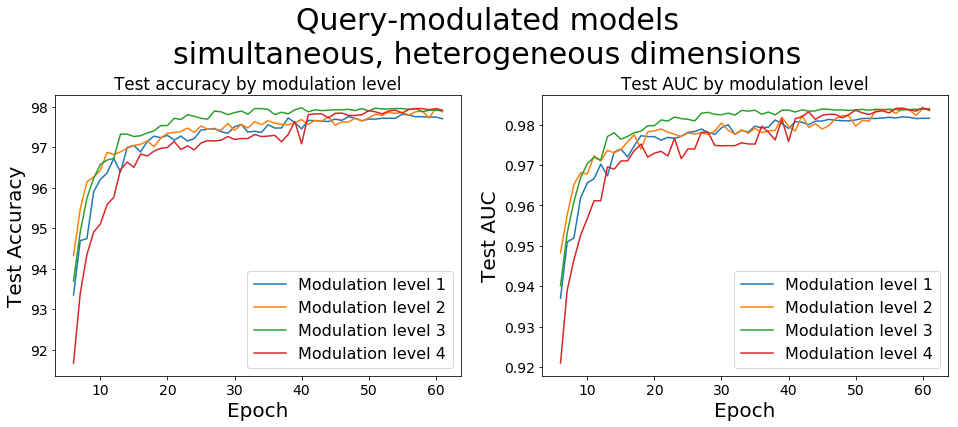
\includegraphics[width=\linewidth]{ch-results/figures/query_mod_simultaneous/query_mod_zoomed.png}
\caption[Zoomed-in version of \ref{fig:results-query-mod-simultaneous-query-mod-only}.]{ {\bf Zoomed-in version of \ref{fig:results-query-mod-simultaneous-query-mod-only}.} To attempt to better distinguish between query-modulated models, we examine them starting from their performance after the fifth training epoch. They still appear very close to even, with a slight advantage starting around epoch 15 to the model modulating at the third convolutional layer group.}
\label{fig:results-query-mod-simultaneous-query-mod-zoomed}
% \vspace{-0.2in}
\end{figure}

\FloatBarrier
\section{Query Modulated Sequential Benchmark \label{sec:additional-figures-query-mod-sequential}}

\begin{figure}[!htb]
% \vspace{-0.225in}
\centering
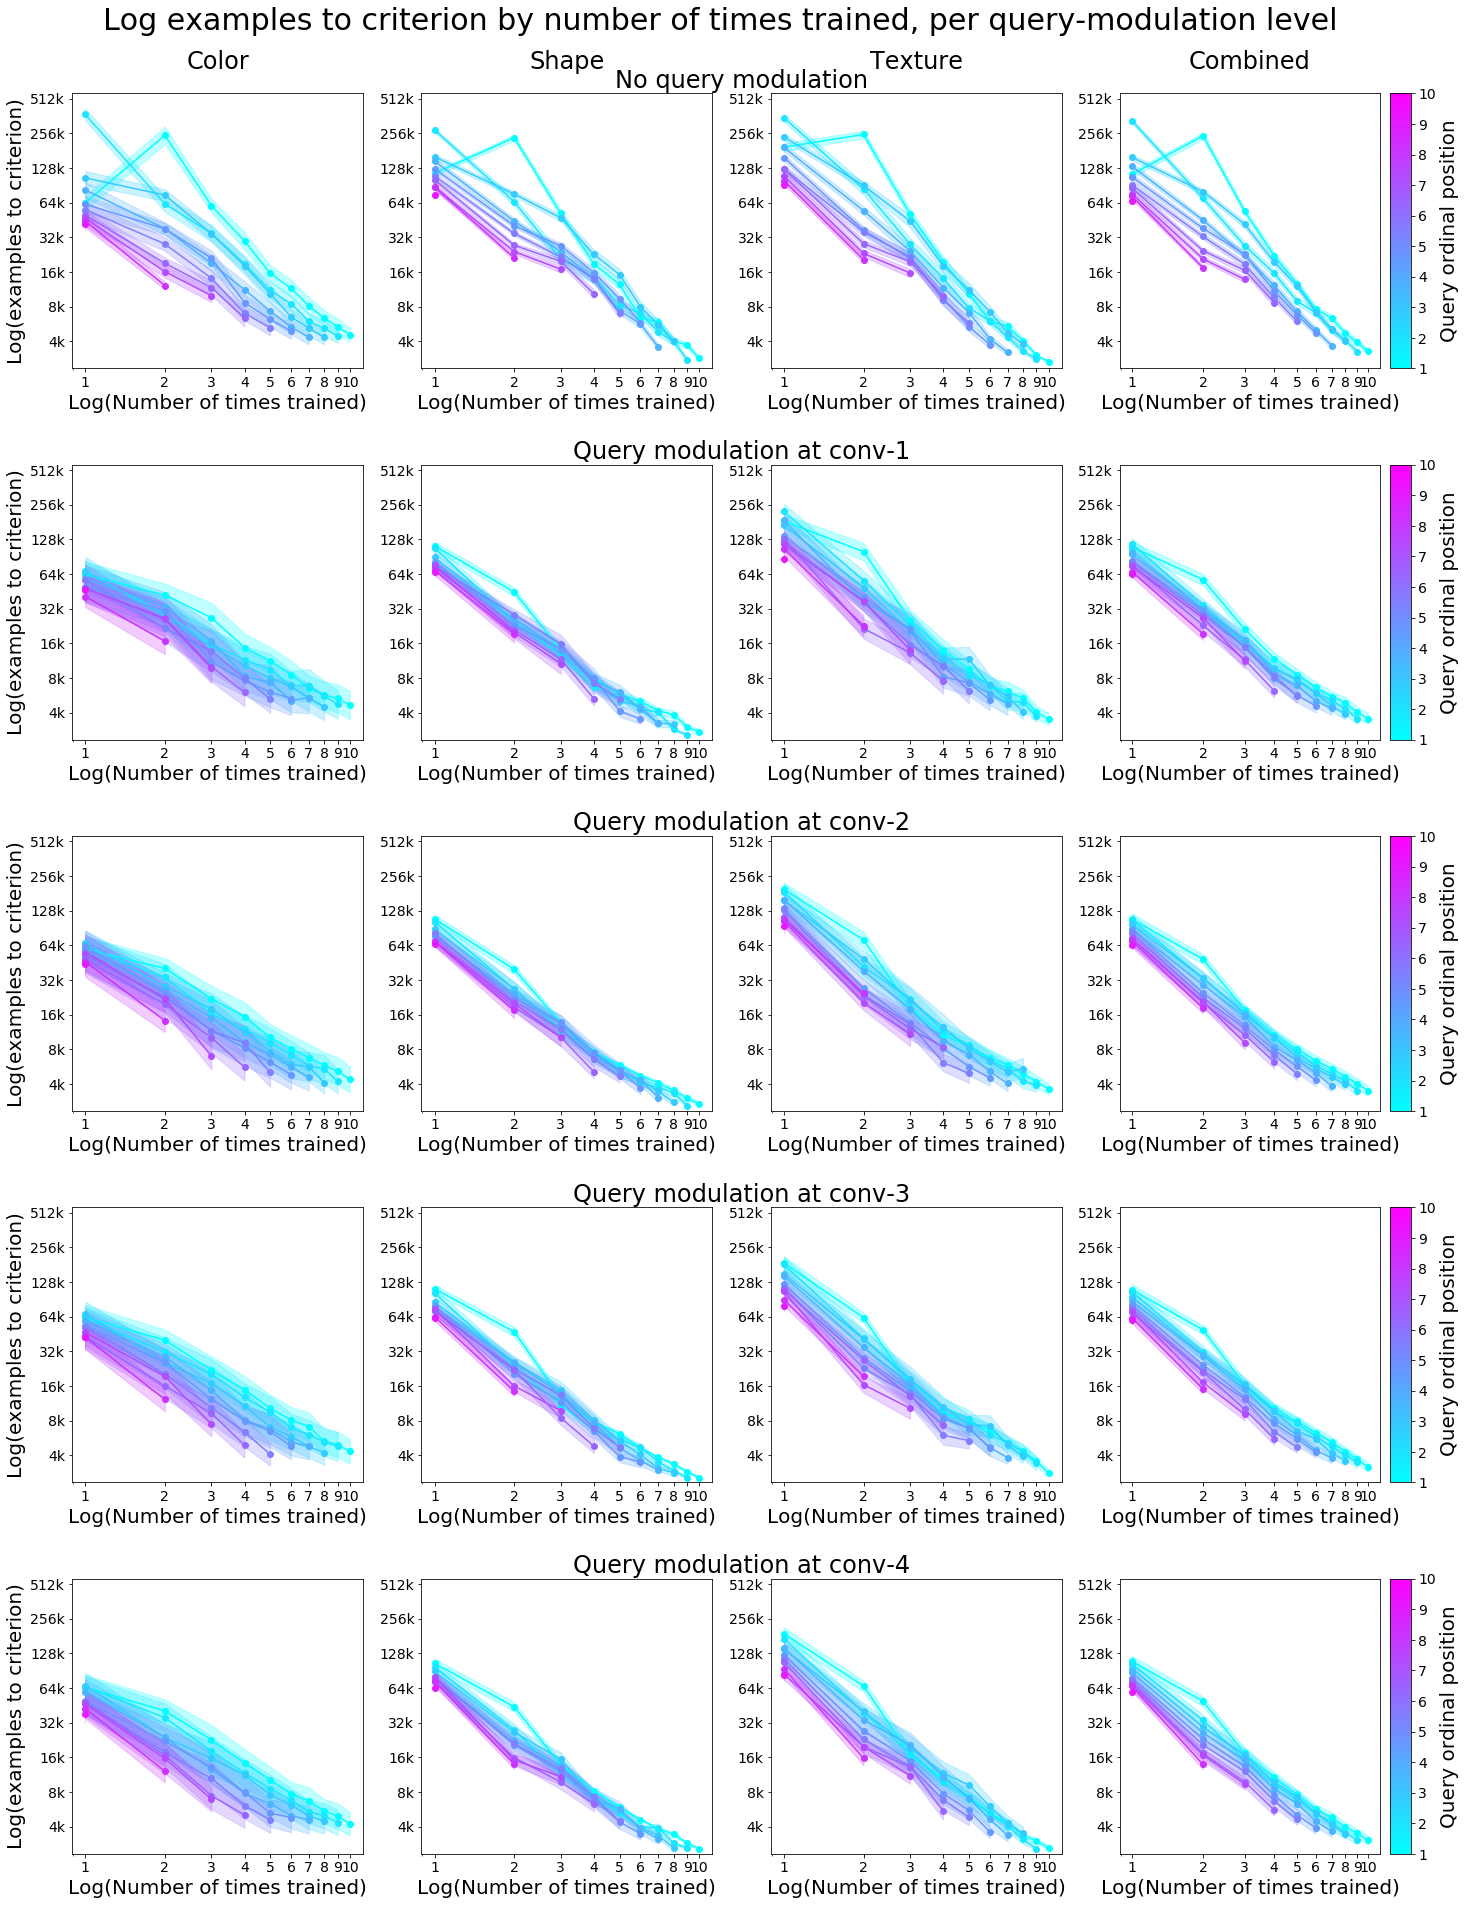
\includegraphics[width=\linewidth]{ch-results/figures/query_mod_benchmark/examples_to_criterion_per_modualtion_level_times_trained.png}
\caption{ {\bf Log examples to criterion by number of times trained.} Split by each dimension and combined. All plots follow the same conventions as Figure \ref{fig:results-baseline-sequential-examples-to-criterion}: using a log-log scale to exhibit the power-law behavior, shading around the data reflects the standard errors of the mean (SEM), and the color scale reflects the order of query introduction, from the first query in the brightest cyan to the last query in the brightest pink.}
\label{fig:results-query-mod-benchmark-examples-to-criterion-per-modualtion-level-times-trained}
% \vspace{-0.2in}
\end{figure}

\begin{figure}[!htb]
% \vspace{-0.225in}
\centering
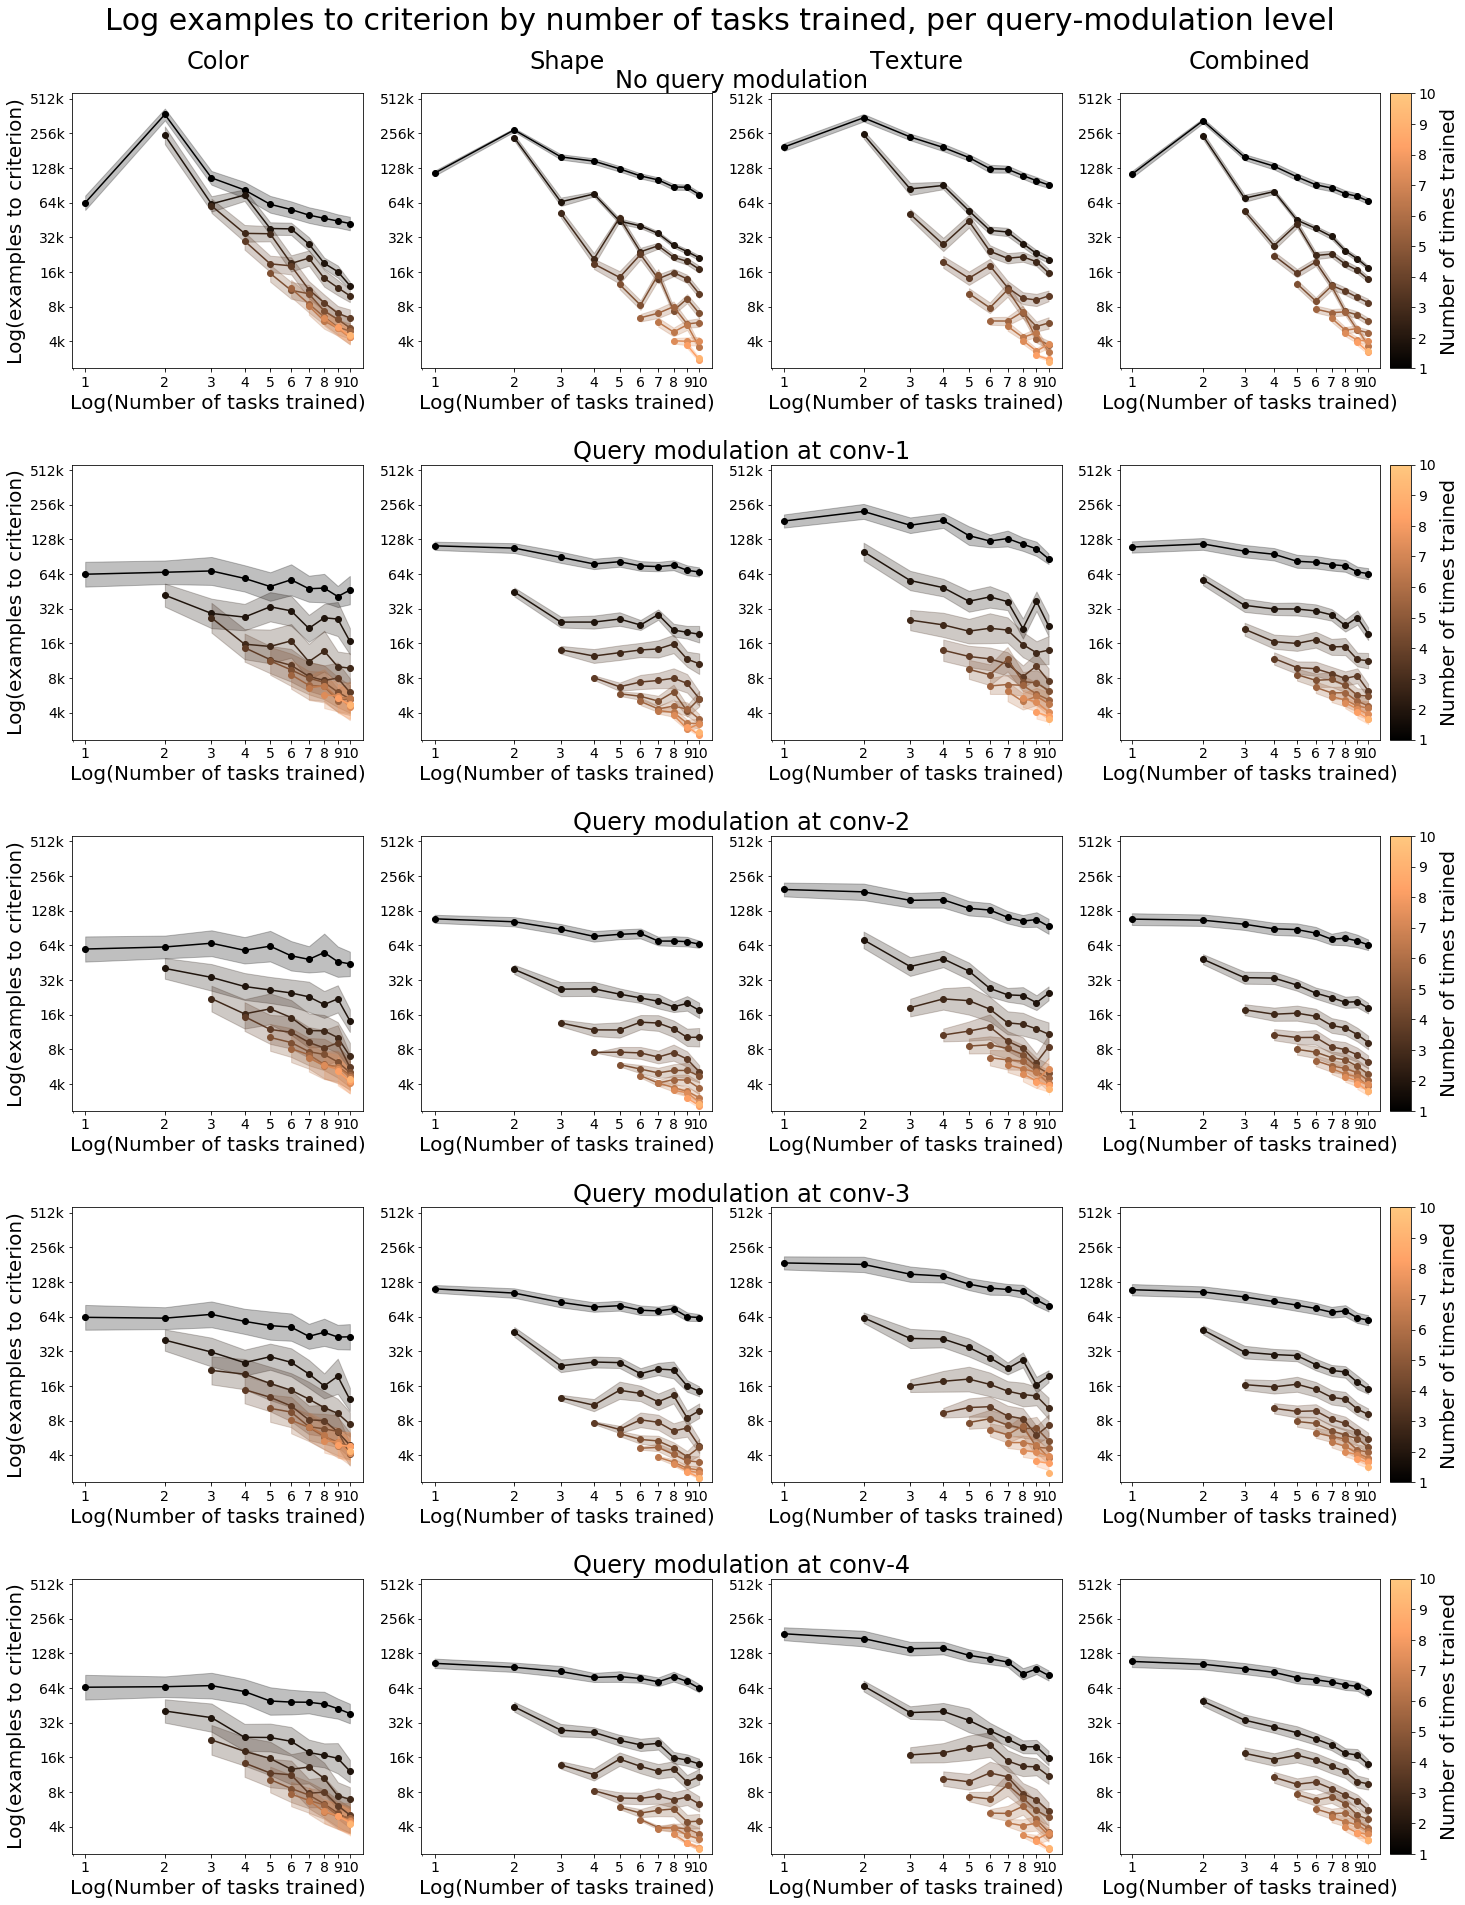
\includegraphics[width=\linewidth]{ch-results/figures/query_mod_benchmark/examples_to_criterion_per_modualtion_level_tasks_trained.png}
\caption{ {\bf Log examples to criterion by number of tasks trained.} Split by each dimension and combined. All plots follow the same conventions as Figure \ref{fig:results-baseline-sequential-examples-to-criterion}: using a log-log scale to exhibit the power-law behavior, shading around the data reflects the standard errors of the mean (SEM), and the color scale reflects the order of query introduction, from queries trained on for the first time in black, to queries trained on for the tenth time in copper color.}
\label{fig:results-query-mod-benchmark-examples-to-criterion-per-modualtion-level-tasks-trained}
% \vspace{-0.2in}
\end{figure}

\begin{figure}[!htb]
% \vspace{-0.225in}
\centering
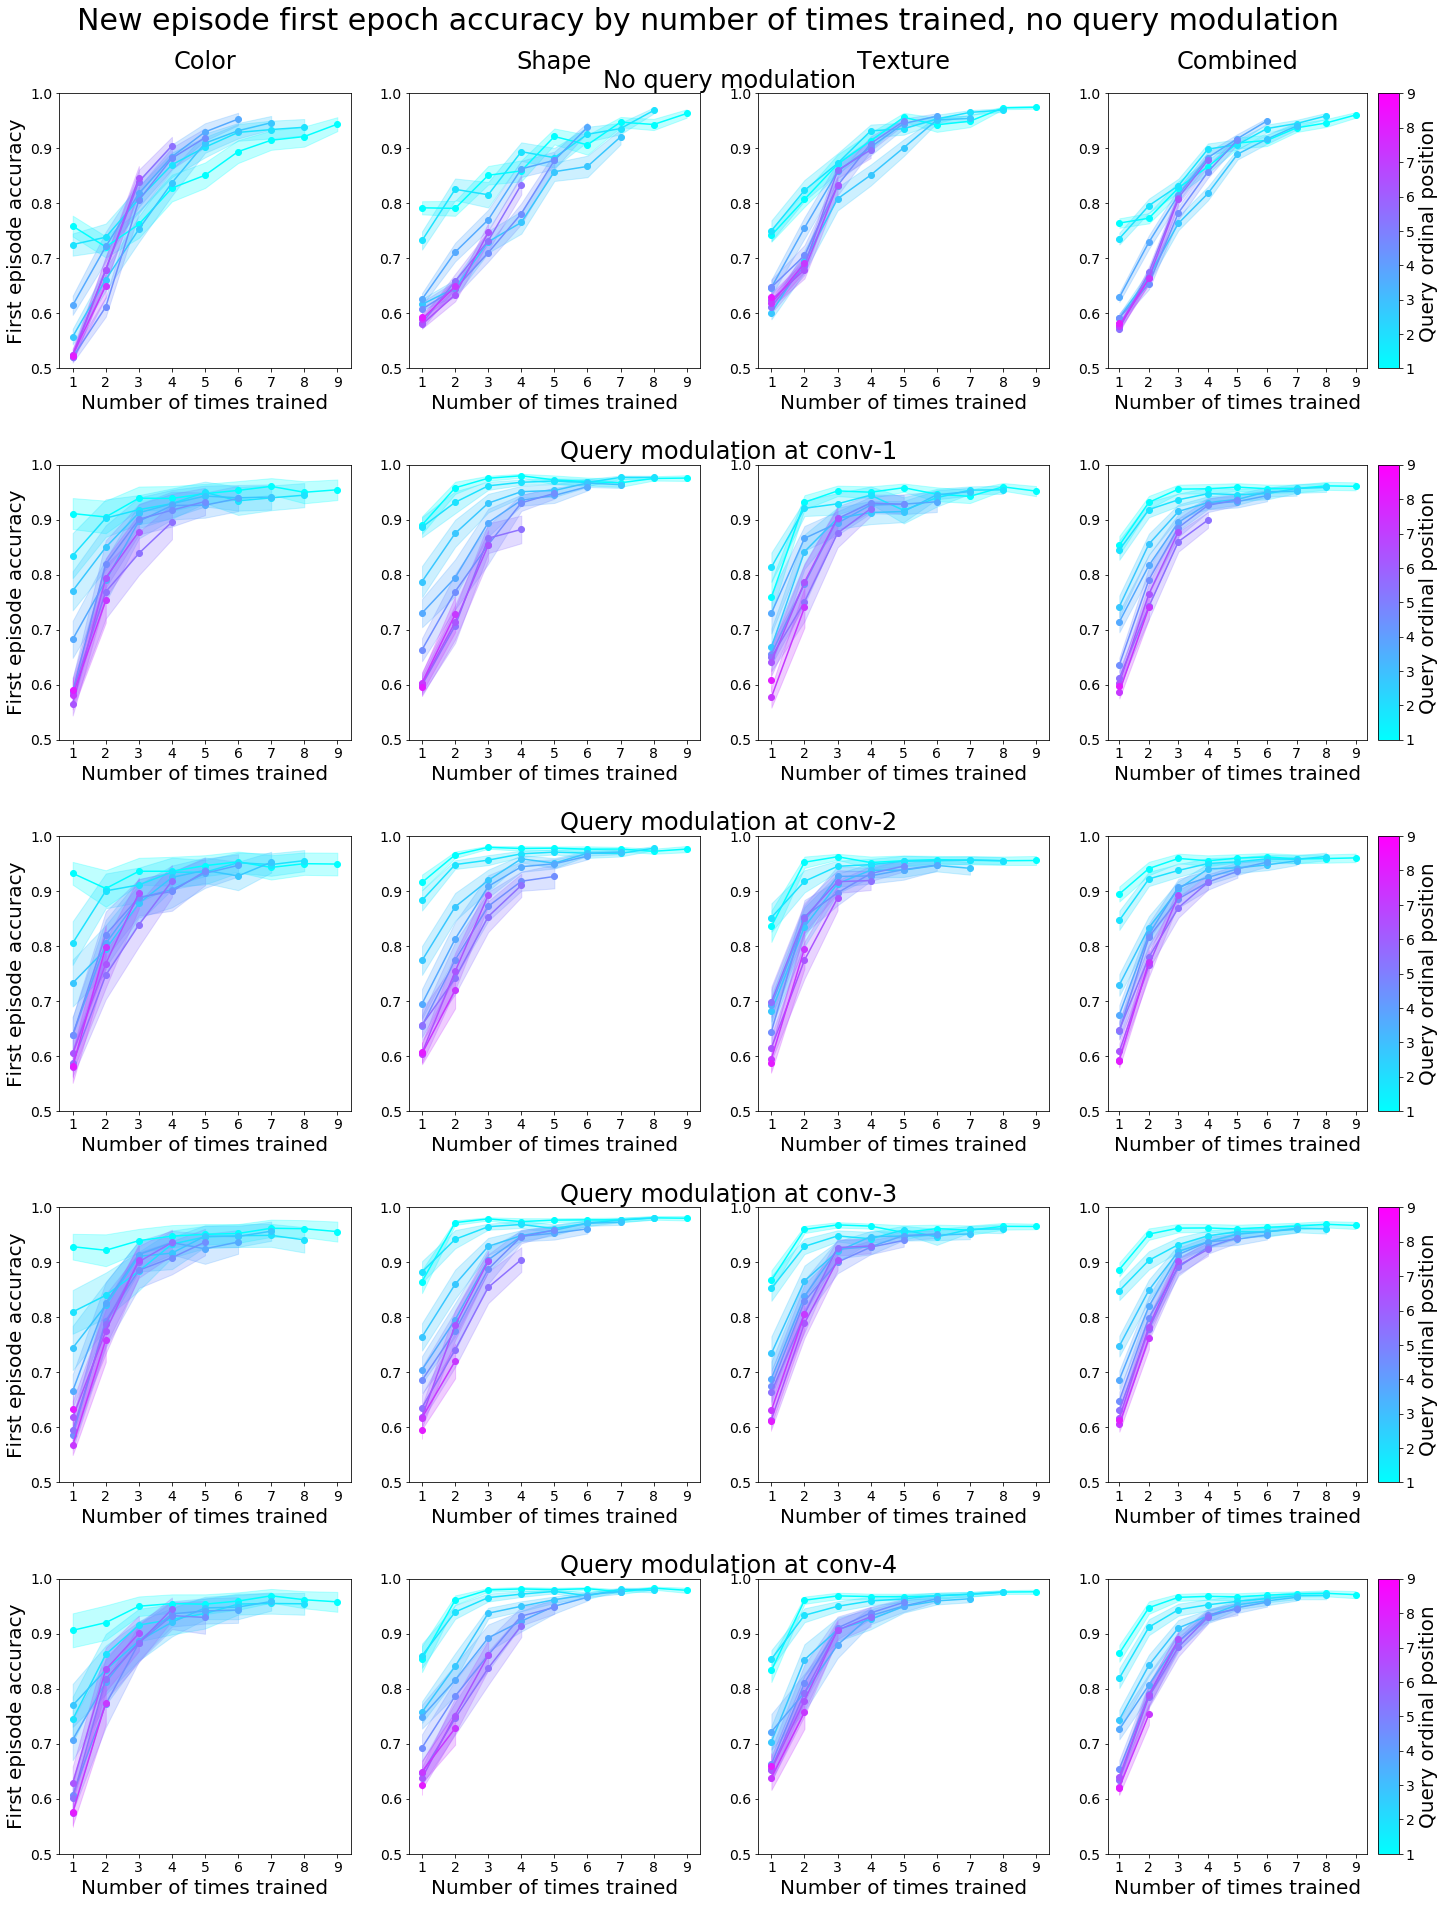
\includegraphics[width=\linewidth]{ch-results/figures/query_mod_benchmark/first_episode_accuracy_per_modualtion_level_times_trained.png}
\caption{ {\bf New episode first epoch accuracy by number of times trained.} Split by each dimension and combined. All plots follow the same conventions as Figure \ref{fig:results-baseline-sequential-examples-to-criterion}: using a log-log scale to exhibit the power-law behavior, shading around the data reflects the standard errors of the mean (SEM), and the color scale reflects the order of query introduction, from the first query in the brightest cyan to the last query in the brightest pink.}
\label{fig:results-query-mod-benchmark-first-episode-accuracy-per-modualtion-level-times-trained}
% \vspace{-0.2in}
\end{figure}

\begin{figure}[!htb]
% \vspace{-0.225in}
\centering
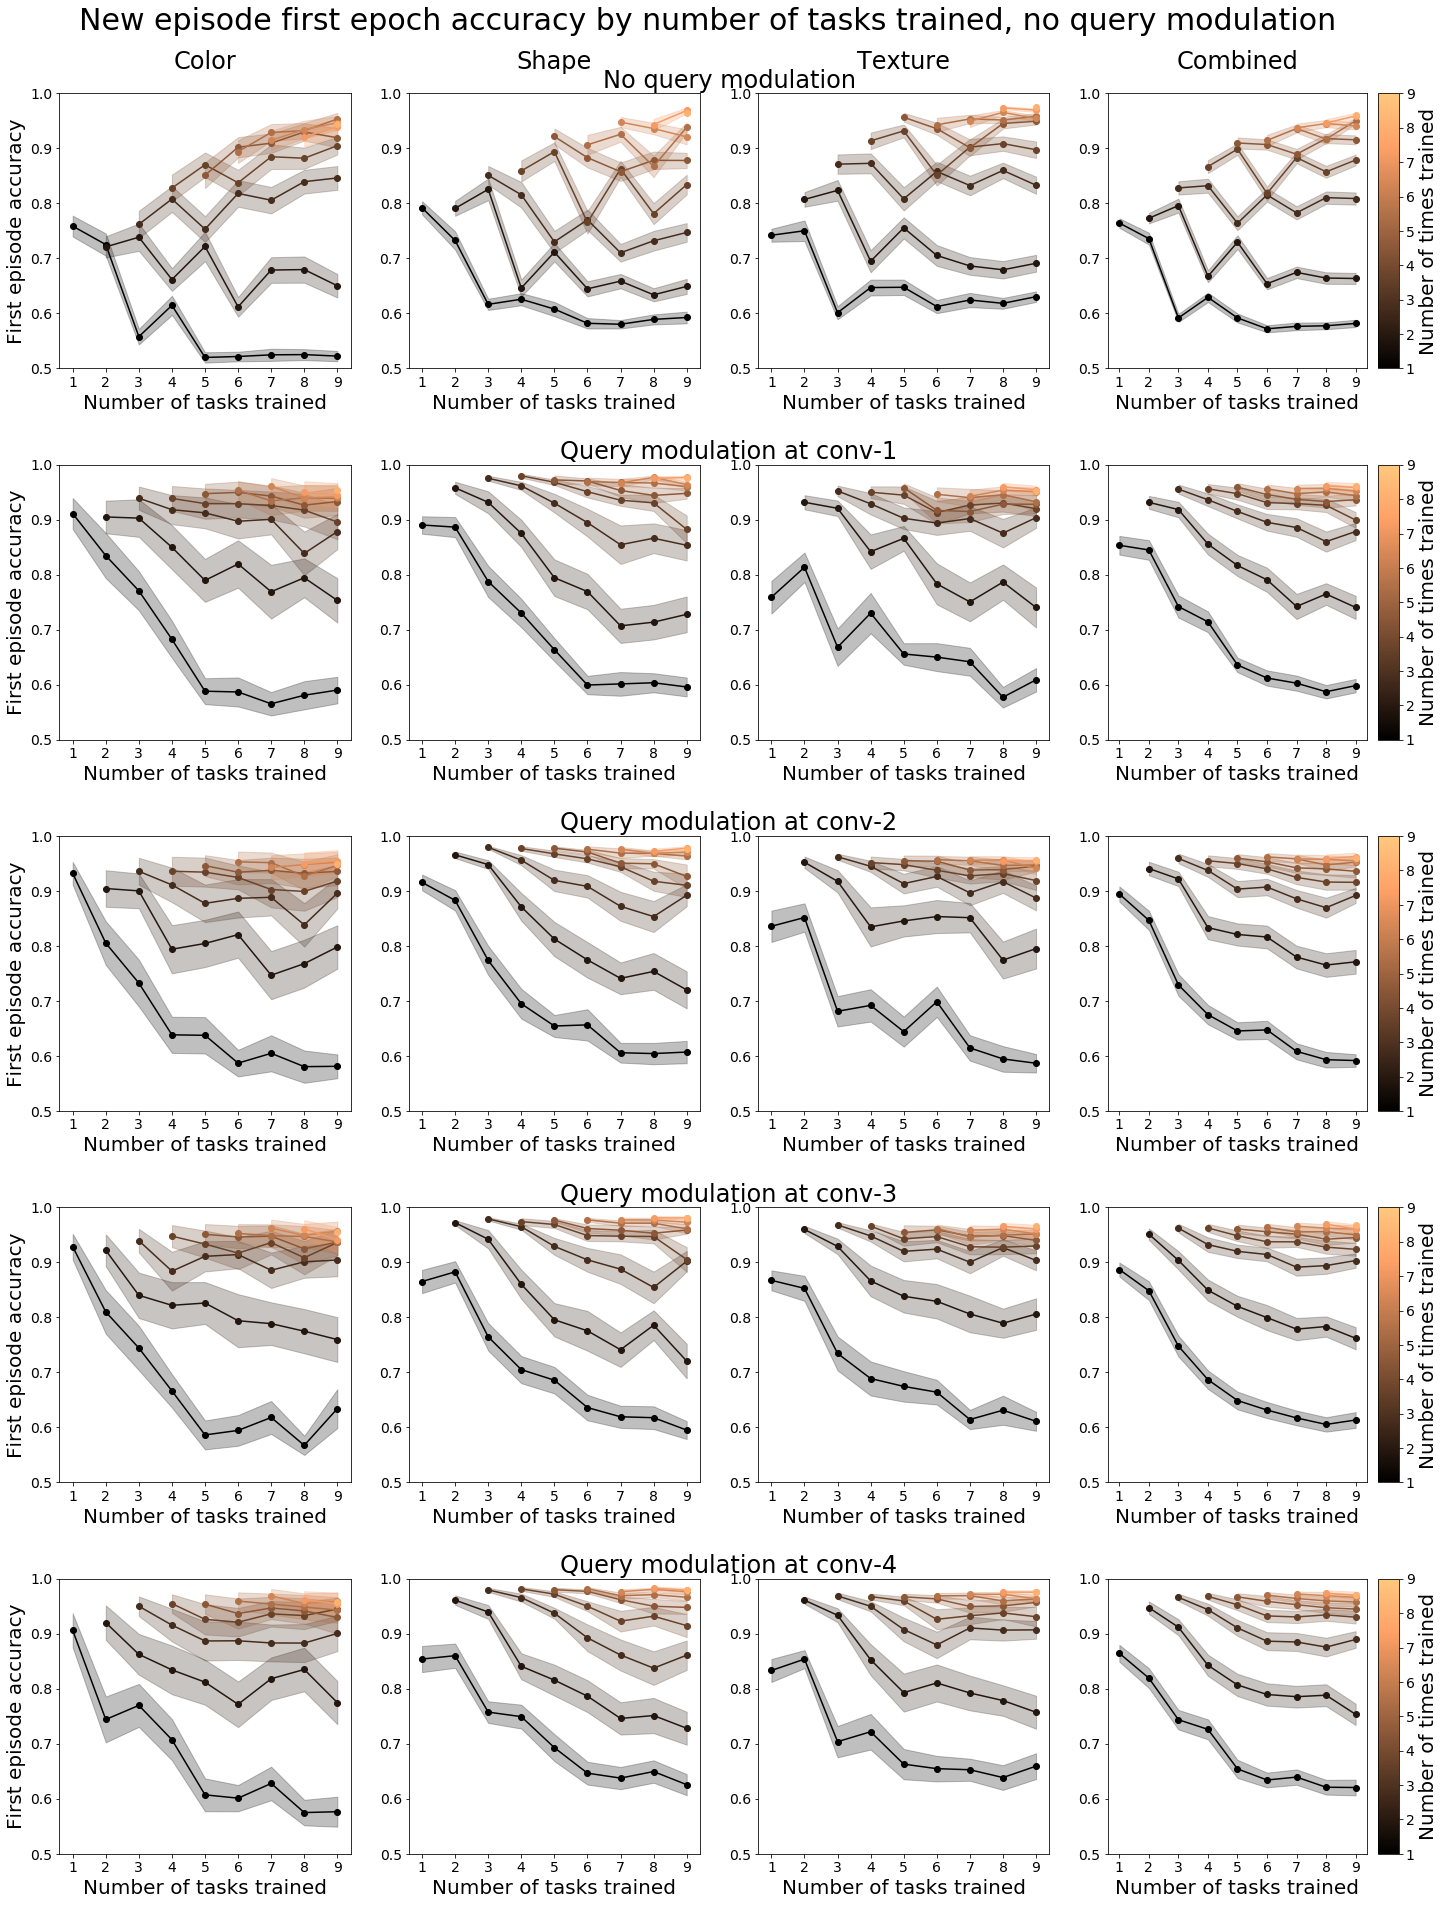
\includegraphics[width=\linewidth]{ch-results/figures/query_mod_benchmark/first_episode_accuracy_per_modualtion_level_tasks_trained.png}
\caption{ {\bf New episode first epoch accuracy by number of tasks trained.} Split by each dimension and combined. All plots follow the same conventions as Figure \ref{fig:results-baseline-sequential-examples-to-criterion}: using a log-log scale to exhibit the power-law behavior, shading around the data reflects the standard errors of the mean (SEM), and the color scale reflects the order of query introduction, from queries trained on for the first time in black, to queries trained on for the tenth time in copper color. }
\label{fig:results-query-mod-benchmark-first-episode-accuracy-per-modualtion-level-tasks-trained}
% \vspace{-0.2in}
\end{figure}



\chapter{Technical Glossary\label{ch:technical-glossary}}

\lipsum[2-4]


\chapter{HC and LO Applications\label{ch:hc-lo}}

\section{Habits of Mind and Foundational Concepts}

\subsection{\#critique}
This work is predicated on a critique of the meta-learning literature. In this section, and in the literature review which comes next, we reviewed a range of works in the meta-learning subfield of machine learning, examining both the proposed methods as well as how they are evaluated. We discovered that the meta-learning attention pays little to no attention to catastrophic forgetting, which motivated the inclusion of literature from the continual/lifelong learning subfield, who do show some concern for forgetting. To provide additional context, we also reviewed some of the older connectionist modeling work from the late 1980s and 1990s. 

Beyond catastrophic forgetting, we discovered that the existing benchmarks in the field do not evaluate the scaling properties of these learning algorithms: how much additional training does a model require to learn a new task, as a function of how many tasks it already knows? How difficult is it for these models to relearn a task, after a later task has been introduced, as a function of how many times the task was previously learned? This critique helped us form the gap analysis which motivates this work:

\subsection{\#gapanalysis}
Two gaps we identified in the meta-learning literature motivate this work. The first is that the meta-learning literature pays little to no attention to catastrophic forgetting. We believe that claims made about how an algorithm meta-learns, or learns how to learn, are only meaningful in the context of retained learning. If we consider human learning to be the hallmark we should strive for (if not surpass), then holding ourselves to a standard of learning quickly and then forgetting is doing us a disservice. In other words, if you cannot show that you retain something you learned, did you truly learn it at all? 

We describe in the end of our Meta-Learning section how few-shot learning inherently introduces some degree of interference, and does not trivially allow to examine how learning scales (and the existing literature ignores this concern). This is not to say that few-shot learning is a useless task. It certainly measures well the capacity of a network to learn how to perform such tasks from minimal information, and with high volatility between each epoch. However, while these models learn fast, they are also likely to forget fast, which this current benchmark does not attempt to quantify. 

Additionally, these tasks do not help us evaluate how learning scales as a function of training. If we begin from the human learner as an ideal, as a person learns how to learn tasks in a particular domain, we expect to see them increasing in efficiency, requiring fewer training examples to pick up tasks as they learn additional tasks. Likewise, we hope that if we train a machine learning algorithm on tasks from the same domain, with sufficient shared structure, the algorithm will improve in its learning efficiency over time. If indeed tasks introduced later require substantially less training to reach an accuracy criterion than earlier ones this would make for a compelling demonstration of learning how to learn.

In the Introduction and Meta-Learning sections, we highlight a gap in the existing literature, and will next describe the solution we propose for it. We start from an existing codebase, which gives us a head start in creating a dataset, and we then demonstrate what sort of adaptations we made and why they were necessary to investigate these properties. We then describe the novel benchmarks we propose to utilize this dataset with, that allow explicitly examining both the scaling behavior of learning algorithms and measuring the degree of catastrophic forgetting they are liable to. 

\subsection{\#hypothesisdevelopment}
The gap analysis presented above motivates the investigation in this work. The dataset, task, and benchmark descriptions below offer our experimental design for how to test these hypotheses. But what, precisely is the motivating hypothesis? 

While we do compare two model architectures, a baseline and a query-modulated processing model, our primary hypothesis is not driven by a belief that one would do better than the other on this task and benchmark (even though we do harbor that belief). Instead, our primary hypothesis is it is worthwhile and meaningful to measure how meta-learning algorithms scale in their training, and how much capable are these models to avoid (or mitigate) catastrophic interference. Because this concern is currently largely ignored, we believe that measuring this capacity on a fairly naive baseline model, without any explicit meta-learning mechanisms, will present meaningful results by itself. It may be the case that this model shows very poor scaling of its ability to learn, requiring similar amounts of training for each additional task, or it could also be the case that this model does show some improved scaling with each additional task from the same domain. Either way, we will be developing a dataset and the methodology to allow exploring these questions, and a baseline set of results upon which other models can attempt to improve. 

It is not the case that we have no prior beliefs on what the results of our experiments will be. For instance, we do believe that even the simplest model will show some improved scaling as a function of the number of tasks and that query-modulated processing will improve upon the baseline results. Rather, our primary and motivating hypothesis is that measuring this scaling behavior and degree of interference will offer a valuable benchmark to quantify the progress of meta-learning research and guide toward more human-like learning. In this sense, it is predicated both on the work on human learning, which shows humans scale learning positively and avoid interference on the level neural network models show, and on the lack of care to these concerns in the existing meta-learning literature. 

On a more meta, research-community level, this work is also predicated on the hypothesis that we are not the only ones who view this consideration as important. If this hypothesis is true, it makes the prediction that we will be able to eventually publish this work, once we complete a few additional steps and write a manuscript to submit to a conference or journal. We firmly believe in this line of work, and this hypothesis creates a very testable prediction, which we hope to be able to report back on in a few months once we further this line of inquiry and reach a publishable point.   

We invoke \#hypothesisdevelopment again in the context of our discussion. The results we observed also motivate future investigations, which we detailed at the end of the discussion. Perhaps the framing we’re most excited about investigating further the stability-flexibility one, in which the model initially learns stable representations, which show lower catastrophic interference but also take longer to learn. As we proceed in the benchmark, and the model learns additional tasks, it changes its representations to more flexible ones, which allow learning new tasks faster, but also show higher degrees of catastrophic interference. Our results so far support this perspective, but we have not yet investigated the nature of the learned representations directly.

If this perspective has merit, the hypothesis is that we would find a way to measure and visualize the representations themselves in a manner conducive to exploring these changes. As the discussion mentions, there is substantial current research on how to visualize the filters and representations learned by convolutional neural networks, but none (that we could find) that examines how these representations change through the course of meta-learning. To begin investigating these hypotheses, we would start by further reviewing the literature on convolutional representation analysis and visualization, to verify there is indeed a gap in the literature. Should such a gap exist, we would then start devising preliminary experiments to run and analyses to conduct.  

\subsection{\#sourcequality}
Beyond strongly situating our analysis of meta-learning and what the field measures or ignores in the literature in the previous section, we took care to perform an additional, thorough literature review. While not encyclopedic, this review encompasses a variety of approaches to meta-learning to situate this work in its context in the field better. Beyond that, we explore influences from visual question answering (which inspired our dataset), human cognition (which helped us design our comparison models), and the lifelong/continual learning literature (which does concern itself with catastrophic forgetting more than meta-learning does).

For this technical glossary, we also sourced references for almost every term. Unlike the main body of the work, which relies on peer-reviewed publications, we understood that a different type of sources fit the purpose of the glossary better. Academic writing is not always optimized for clarity, and peer-reviewed publications are usually aimed at domain experts, allowing the writers to avoid elaborating on most concepts. We, therefore, opted to go for a collection of blog posts, Medium articles, tutorials, and course notes, all of which assume substantially less knowledge and provide more lengthy and understandable explanations. We hope the readers find these sources useful.

\subsection{\#audience}
We aim this work to be understandable to a technically savvy audience with no particular machine learning background, besides having probably heard the term at some point (given it is nigh-impossible to read anything technological and not encounter it. To that end, we wrote an extensive technical glossary, introducing general machine learning terminology, fundamental concepts relevant to neural networks, and particular concepts that are relevant to the dataset and task we created. The hope is that adding these elaborations helps readers who might be familiar with some terms but not others get up to speed on relevant concepts to this work, and improve the ability to understand our technical methods and contributions.

\subsection{\#testability}
Given the description of the hypothesis above, it does not lead to testable predictions of the form “these model would do better than that model under such conditions,” but it does lead to an overall testable form for the work. We make a claim (the hypothesis) that these concerns merit investigation, and can be interrogated well. To test this claim, we need to clear two hurdles. 

The first hurdle is the ability to measure the scaling properties of these different models as a function of learning. The next entry will describe the dataset, task, and benchmarks we develop, which allow to investigating these properties explicitly. We designed an experiment allowing to control for many irrelevant factors, and by that standard, if we can develop an experiment to measure this form of behavior, it is testable. However, our hypothesis was not that this behavior is measurable - we assumed that we could devise a dataset and paradigm that would allow measuring these qualities. 

The second hurdle is the ability of this experiment to generate meaningful results. As evidenced by the fact we are reporting these results, we believe they offer insight into how these (somewhat naive) models scale in their ability to learn as a function of the number of related tasks they already learned. If, for instance, all of the models we evaluate score similarly on the benchmarks, it is either the case that (a) these models are functionally equivalent, in their ability to scale learning and avoid forgetting, or (b) that this benchmark does not evaluate what we had hoped it would evaluate. In other words, the testable prediction is that different models will perform meaningfully differently on this benchmark if we design it well from an experimental perspective (see the next HC note). 

\subsection{\#interventionalstudy}
The construction of the dataset allows us to investigate a number of properties, and the different benchmarks are experimental designs that use this dataset to investigate a particular characteristic we hope to find in meta-learning algorithms. We evaluate a baseline model to establish an expectation and understand what sort of behavior we should expect on this benchmark from a reasonably naive model. We then compare it to a few different variants, which serve as the experimental conditions in this design. The dependent variable we wish to evaluate is the performance on this benchmark, both in how quickly the model learns all ten tasks to criterion and in what the scaling behavior is for the amount of training required for each successive task.

To minimize the effects of extraneous variables, we attempt to control for as many of them as possible. Having noted that the different dimensions (shape, color, and texture) show varying degrees of difficulty, we treat them separately and consider replications over the benchmark in the ten tasks of a single dimension, rather than over all thirty single-feature tasks. To account for order effects, of particular task orders being easier to learn than others (perhaps, hypothetically, it is easier to learn to recognize cubes before spheres than the other way around), we employ a Latin square design, which guarantees that within each block of ten experiments, each task will appear in each ordinal position (first through tenth) exactly once. We perform a few replications of these ten-experiment blocks to increase the robustness of our results. We fix all random seeds, such that the training set is presented to the model in a consistent order for every task replication.

We follow similar principles with the design of the dataset. While we added substantial variation over the original CLEVR dataset in the colors, shapes, and particularly the textures we used, and we randomize the positions of the objects within each image, we decided to hold most other visual factors constant. We removed any jitter in the orientation of the objects, such that other than any minor occlusion, they always appear the same in every image. We similarly eliminated randomization in the location and angle of the camera relative to the objects, and in the location lighting during rendering. If we eventually discover this dataset is too trivial, we can easily reintroduce these factors, but for the time being, removing them allows us to focus on the learning tasks. 

\subsection{\#variables}
The formulation of the benchmarks and experiments is centered around our identification of the relevant variables. In this case, we treat the choice of model as our independent variable, which allows us to compare performance on different models. The direct dependent variables we measure are the accuracy on every query in the benchmark, and how many training examples it takes the model to reach the accuracy criterion for every task. To evaluate the models, we then aggregate these measures by how many times a query was trained on, and how many total queries the model knows, and arrive at plots that allow us to holistically evaluate the scaling behavior and catastrophic forgetting we wish to use to compare models.

We also knew there is a number of extraneous variables we want to control for. We initially separated the results by dimension, to be able to demonstrate that they qualitatively behave similarly, even if some dimensions are harder than others for the model to reason in. We compared the models on identical query orders, to make the comparison valid. We used a Latin square design, which guarantees that over a block of ten queries in a dimension, each query will fall in all ten ordinal positions, mediating order-related effects. We fixed all random seeds, to attempt to remove randomization-related variance. 

We later realized that our choice of introducing queries from a single dimension is itself a variable we can compare on, and so we designed the control (sequential, heterogeneous dimensions) condition to provide an alternative case. When designing that case, we wanted to account for order-related effects as we did before, but this time between the dimensions. To do so, on every control iteration we pick one of the six permutations of the dimensions and sample a query from each dimension until we reach ten queries (to match the sequential, homogeneous dimension condition, which has ten queries in each dimension). This method of selecting the query order makes the control condition maximally different from the regular sequential one, using three to four queries from each dimension, and maximally spacing the queries from each dimension.

In summary, our experimental design took under consideration every variable we identified and could reasonably control for, allowing us to us to focus on comparing different model variants on how well their learning scales and how much catastrophic forgetting they exhibit or comparing the same model in different experimental conditions. In both cases, our independent variable is categorical, while our dependent variables are the quantitative measures we make of the model. To compare, we, therefore, devised plots that explicitly examine the dependent variables for a pair of independent variable settings (see the \#dataviz section below), and performed a statistical sign test on the differences between these models (see the \#significance section below).

\subsection{\#algorithms}
As the annotations above describe, we wrote substantial amounts of code for this project. In many cases, we found that an appropriate choice of algorithm, or especially data structure, can both substantially simplify and accelerate the code. Here are a few examples:

We saved cached results of long computations in a few places, rather than repeating them every time. We did this with the normalization of the dataset, saving the mean and standard deviation in each channel, rather than computing it from the 45,000 image dataset every time we repeated the benchmark (see \texttt{dataset.py:create\_normalized\_datasets}). We similarly saved the processed versions of experiment results to a (separate) cache, rather than querying the Weights \& Biases API and preprocessing anew if we wanted to explore the results in separate notebooks or needed to restart the kernel (see the notebooks whose names end with `\texttt{plot\_experiments.ipynb}' and `\texttt{benchmark\_final\_plots.ipynb}').

We also performed similar caching in our dataset class for the sequential benchmark (\texttt{dataset.py:SequentialBenchmarkMetaLearningDataset}), storing for every query, which images should return true and which ones should return false. We use this data in order to allocate the coreset, which changes every epoch. While we initially first allocated the half assigned to the current task, and only afterward the half assigned to the coreset, we discovered that this order sometimes leaves us with imbalanced data in the coreset, with some previous queries receiving too high a proportion of negative or positive examples. To remedy this, we flipped the order, first allocating examples to the coreset, verifying that each task receives a sufficiently balanced set, and only then assigning the remaining examples to the current task. We reasoned that having a large number of examples assigned to the current task would leave us much less likely to receive an imbalanced subset. 

In this allocation process, we also ran into another issue. At some point, we discovered that allocating tasks to the coreset takes about two minutes, which is longer than what the rest of an iteration through the benchmark (training and testing) takes. We initially had the aforementioned positive and negative images for each task stored in lists, since numpy’s sampling algorithm can sample from lists (and other index-able data types). However, when we then searched for specific examples in these images, we were incurring a linear-time cost, since searching in an unsorted list takes $O(n)$. We realized it would be much wiser to hold these collections on images in sets, which are hash-backed, and therefore allow $O(1)$ searching. The penalty of converting between sets and lists a few times was dwarfed by the benefits from optimizing the search process, and so we repeated this logic in another place in the same function and saw substantial speedups (\texttt{dataset.py:SequentialBenchmarkMetaLearningDataset:start\_epoch}). 

\subsection{\#dataviz}
We created a substantial number of data visualizations to aid in interpreting our results and metrics. Some of our plots are fairly standard, describing the performance of a single model, or group of comparable models, using overall metrics (such as the loss, accuracy, or ROC AUC). Some of our panels depict more complicated behavior, such as the results for each query-modulation level within each query, split by dimension, to allow examining how behavior changes between models and different types of queries. Our most nuanced visualizations present our measures of learning scaling and catastrophic forgetting, as a model accrues additional experience on a given query or the entire domain (a dimension). We also modified these plots to explicitly compare between a pair of models, simplifying comparative evaluation. 

In all plots, we took care to use the appropriate scaling, changing between logarithmic scaling and linear ones based on what made the most sense. We offered axis legends to ease interpretation, as well as color bars to clarify the meanings of the color scales used. Where appropriate and available, we shaded the standard error of the mean around our data, to provide a measure of uncertainty. When a clear reference point exists, such as an accuracy threshold or a baseline difference or ratio, we plotted it as well.

Our results section presents these results, and our discussion section analyzes them. We believe that these data would be harder (if not impossible) to interpret if we tried to condense them to single numbers. We find these plots useful, and they both reveal insights on the data and motivate the discussion and some of the future lines of inquiry suggested.

\subsection{\#induction}
Machine learning models generally, and neural networks specifically, all reason by induction, learning to map patterns and correlations between the inputs and outputs. For this reason, we measure neural networks not by their capacity to perform on the data they observed and trained on, but their ability to generalize to new data, in a test set, on which the model is evaluated but not allowed to learn from. The premise of this work is that when we evaluate meta-learning, the capacity of a model to learn to induce correctly in a new task, we should examine how the learning scales, to see if the model learns to perform inductive judgments faster as it receives additional training. We should also measure catastrophic interference, how much does new knowledge interfere with previously learned inductive judgments. 

We end up identifying that some inductive problems are inherently easier for the models we examined than others -- colors were the simplest, save for two colors which turned out to be perceptually confusing; shapes were also relatively easy, and textures required the most amount of training learn to generalize on correctly. From the control (sequential, heterogeneous dimensions) condition, we learned that our model’s improved scaling is not as much about accrued expertise within a domain, as the control condition showed comparable scaling and weaker interference patterns. We similarly discovered that our alternative, query-modulated model shows slightly better scaling, but most predominantly shows weaker interference patterns. 

It is interesting to note that we do not usually consider interference between old knowledge and new knowledge in humans performing inductive judgments. \textcite{Gopnik} and \textcite{Griffiths2011} investigate the effects of knowledge on causal reasoning in children, but not directly in the context we postulate here. It stands to reason, though, that if a child were learning to identify birds, a simple criterion they might use would be that birds are flying creatures. Once introduced to bats, and told they are not birds, but mammals, the child might confuse other birds as mammals, until developing more exact criteria, that allow recognizing bats (and other flying mammals, such as flying squirrels or flying lemurs\footnote{\url{https://www.quora.com/Why-are-bats-the-only-flying-mammal}}) as mammals. We are not aware of any cognitive or developmental psychology literature examining how human induction judgments change when additional information is presented or new tasks introduced. From a Bayesian perspective, we can consider an abstract hierarchical model, where each category is defined by the parameters of a distribution in a high-dimensional latent space, from which we can sample examples, and as we learn to label these examples, we update our posterior notion of the distribution in the latent space. Learning that not all flying creatures are birds might initially cause too stark a shift in these distributional parameters, which would be eventually remedied as the parameters are refined through additional examples. 

\subsection{\#significance}
For the most part, we provide evidence for our results through visualizations, which we find work better for presenting and comparing the results of these models than statistical tests do. However, to also provide a statistical measure of the differences between the models, we perform sign tests on the results, examining both which models reliably require fewer examples to reach criterion, and which models show lower effects of catastrophic interference. To increase the robustness of the results, we repeat the tests while accounting for the standard errors of the mean (SEM) around each per-model average, such that we only consider differences that are not within their respective SEMs. While not a measure of practical significance per se (as we did not compute a measure of effect size, as those are incompatible with sign tests), it does help points to results that are likelier to carry practical significance, in the sense that if we repeat these experiments, we will have a stronger belief that the SEM-corrected comparisons will replicate than the non-SEM-corrected ones. Additionally, if the results do not have overlapping SEM intervals, they must be farther apart, and therefore likelier to merit practical significance, although, we did compute a measure of effect size, as no such measure exists for this sign test. We can also view this correction as reducing the power of this test to detect an effect, but increasing its robustness. When using the SEM-based correction, we reduce the probability of false positives (type I errors), as we avoid counting some differences that are below the SEMs; but we increase the probability of false negatives (type II errors) by making the bar higher. 

\subsection{\#scienceoflearning}
A recurring motif in our discussion is the use of similar examples from cognitive psychology and the science of learning to help interpret our results and our model’s performance. When we designed the task, we realized we have to include a coreset of examples from previously trained tasks, and in fact, that it is insufficient to merely train on them, but that if we want to guarantee the model retains them, we must also make them part of the accuracy criterion to be met before a new task is introduced. We then realized that this resembles the notion of distributed or spaced practice for human learners, where students are encouraged to continue practicing previously learned materials, increasing the temporal distance between repetitions of previously acquired knowledge as it becomes better cemented. This parallel to spaced practice, of continuing to train and test on previous tasks, proved crucial to the ability of our model to learn the benchmark, as the plots in the benchmark formulation section demonstrate.

Under this interpretation, though, our method of allocating coreset examples is unideal. We currently allocate half of the examples in each training epoch to the current task, and the other half, which we term the coreset, to all previously learned tasks. The examples in the coreset are allocated evenly between all previous tasks. To see why this may be unideal, consider the training of the tenth (and last) task in an iteration of our sequential benchmark. Each of the previous nine tasks receives $22,500 / 9 = 2500$ training examples, even though the first task is being learned for the tenth time, while the ninth task is only learned for the second time. Since we train on every task in every epoch, our analog for the temporal window in spaced practice is the number of examples allocated in each epoch. 

If we wanted to take on a strategy that more closely matches the recommendations of the cognitive psychology literature, we could change the coreset allocation, such that tasks receive training proportionally to how many times they have been relearned. Presumably, the freshest tasks might require the most amount of continued training, which we can also see in the catastrophic interference results - tasks learned for the first time show the strongest interference once the next task is introduced. We could change the coreset allocation from evenly allocating examples, to allocation proportionally to the number of times a task has been retrained. To measure the effectiveness of such a strategy, and compare it to the current one, we could count the number of `wasted' training examples, which we would define as training examples allocated to a task which is currently above 95\% accuracy. The hypothesis would be that a less naive allocation system, which draws on the science of learning, would ‘waste’ fewer examples. Note that these examples still help the model train, as there is still a loss unless the model allocates the full probability mass to the correct answer, but they do not help the model finish the current stage of the benchmark sooner, as the task they are allocated to is already above the accuracy threshold. 

\subsection{\#professionalism}
We went through the trouble of converting our draft from a Google Document to LaTeX, in order to adhere to a professional standard for a thesis and verify our work looks as clean and elegant as possible. We also recreated several visualizations we had in the Weights \& Biases service using matplotlib, to ensure consistent visual style within all of the plots presented, as well as allow us additional control over the sizes of labels and legends. We also make the entirety of our work open source and document it well, to allow other members of the research community to explore and interact with our work, verify our results, and extend it should they choose to. 

\subsection{\#organization}
We follow the standard form for presenting a research paper in this community. We begin with an introduction, which broadly surveys the field and presents the main line of inquiry we pursue. We follow that with a detailed analysis of the meta-learning literature, which helps identify the gap we explore and how existing work interacts with our ideas. To provide additional context, we offer a broader review of the literature, examining various approaches and better situating our work. We then outline the work we did, starting with the generation of our dataset and formulation of our benchmarks, and following that with a thorough description of the models we compared. We describe our results, offering data visualizations and tables where relevant. We conclude with a discussion, which summarizes our contributions, offers our interpretation of the main finding, and concludes with our plans for future work in this topic. 

\subsection{\#evidencebased}
We attempted to be rigorous and thorough with our use of evidence across this work. To make the case that the existing literature neglects our concerns, of scaling behavior and catastrophic interference, we reviewed it extensively, eventually delving into a second field (lifelong/continual learning) in order to provide additional context on those concerns. To elaborate on the importance of examining these properties, we draw on human learning, which serves as a standard for what learners might be able to do, and we discuss why scaling positively is an important concern for a true meta-learning model, an algorithm that learns how to learn. In the results, we try to back our claims with multiple perspectives on the same evidence, plotting our key figures aligned two separate ways, both by the number of times a task was learned and by the number of tasks a model knows, in order to further illuminate our results. In our discussion, we offer the perspective of examining this model through the stability-flexibility tradeoff often discussed in biological memory, and provide a number of arguments for what that perspective is reasonable to take and well-supported by the results, and useful, in the sense it offers a meaningful interpretation of the results and guides toward future work. 

\section{Learning Outcomes}

\subsection{Capstone \#metalearning}
Components of the application of this learning outcome for the capstone project stem from the HCs detailed for this section and the next several ones. We believe that our analysis of the field of meta-learning was sound, and allowed us to offer a novel perspective on the problem of meta-learning, by suggesting to examine both the scaling of learning and the prevalence of catastrophic interference. The former of these is effectively ignored in the meta-learning literature, while the latter is mentioned in passing. We developed metrics and plots that allow examining and visualizing both, which we will showcase in the results section. In this section, we design a dataset and task setting and propose two benchmarks that allow empirically exploring these concerns. The next sections of this paper will explore the models we compared, the results we collected, and a discussion of the implications of our findings and relevant next steps to explore.

\subsection{CS156 \#classification}
We compared the task paradigm we proposed to several other supervised learning, computer vision paradigms, and explicitly drew out the differences in order to explain why we consider it a meta-learning problem, and how it differs from existing tasks investigated in the field. The rubric for this LO offers the possibility of “analyzing, explaining, or justifying the application in a way appropriate to the given context.” The description in this setting serves as the analysis and justification of why we treat our problem as a supervised classification problem and employ similar methods, explicitly noting it can be viewed as a logistic regression problem from [image space] X [query space] to a binary label. The models compared (below) offer an implementation of neural network models for this precise setting. Note that both the activation function we used on the last layer of the models (the log-softmax function) and the associated loss function (negative log-likelihood, related to cross-entropy) are standard choices in classification paradigms, further reinforcing the connection to classification problems. Additionally, the standard error metrics we will report, accuracy and ROC AUC (Receiver Operating Characteristic Area Under the Curve) are standard choices in classification settings.

\subsection{Capstone \#datasetsandbenchmarks}
We developed a novel dataset tailored to allow investigating the sort of questions we would like to ask. We started from the CLEVR dataset and their open-sourced generation code and modified it heavily for our purposes. As detailed in the section, we added colors, object shapes, and a variety of textures (materials), allowing us to have ten unique queries in each dimension, creating symmetry between them. We then reduced other sources of visual variance, such as jitter in the location of the camera and orientation of the object, to simplify some components of the visual challenge. We noted that if it proves overly trivial, we can introduce them later, but reasoned that removing these types of noise will help us focus on the questions we want to ask.

We then suggested two novel benchmarks with this dataset, implementing one in this work and leaving another for future work. These benchmarks employ the characteristics introduced in the dataset, allowing us to examine the performance when all tasks introduced are in the same dimension (homogeneous dimension), and later, as a control, when the task introduced vary between the dimension (heterogeneous dimensions). Introducing the tasks sequentially allows us to examine how learning scales as a factor of two variables: first, by how many times the model was retrained on a particular task, and second, by the order in which the tasks were introduced, which corresponds to how many tasks the model was training on at that point in time. We similarly examine how catastrophic forgetting varies by these two variables. Effectively, the first measure allows us to quantify if what is helpful is practice on a given task, and the second measure if what is helpful is experience with a given domain (in this case, a particular dimension). We will report in the results plots allowing to examine both of these types of scaling, both within a single model, and comparing a pair of models, creating a standard to which we (and other members of the research community) can compare additional models to in the future.

\subsection{CS156 \#neuralnetworks}
We picked a neural network design appropriate to the context and task it is solving, similar in design to models used in the literature. We justified both its use and the modifications made by introducing query-modulated visual processing to this task. We believe our baseline models makes for a reasonable standard for comparison, and our query-modulated design is the minimally-complex sophisticated design that might show better performance and operationalize the ideas we had in mind. We implemented these models in PyTorch and compared them extensively in our results. We believe our review of the literature should serve as sufficient evidence that there is no simpler model we could have tested and expected to perform equally well on this task. 

\subsection{Capstone \#softwareimplementation}
We implemented the models, dataset generation, benchmarks, and analysis and plotting code in Python. While we developed different parts of the codebase to slightly different standards, we attempted to follow best practices for research code in all code written. Variable names were chosen to be consistent and clear. Code reuse was encouraged by splitting functions at appropriate boundaries, and using inheritance in most places it was sensible. Most functions receive optional arguments to flexibly allow for multiple behaviors with the same underlying logic. Each folder offers a readme, and most functions are documented, offering a description of the purpose of the function as well as the essential inputs and the format of outputs. 

The code is still research-level code, rather than production-oriented, so it is imperfect at times. We did not implement any unit tests, although we manually tested the behavior of most of the code. There exists some code duplication in cases in which it was easier and faster to duplicate some logic rather than abstract it out; this is a clear minority of the code written, but it still exists. Overall, we are proud of the code we wrote for this project, and are happy to have it representing us on GitHub. 

The main package of research code is here: \url{https://github.com/guydav/deep-learning-projects/tree/master/projects/metalearning}
The analysis and visualization code and notebooks using them are here: \url{https://github.com/guydav/deep-learning-projects/tree/master/notebooks}
The dataset generation code, which is less polished, as it is forked from the original CLEVR-dataset-gen repository (which is not very elegantly written), is here: \url{https://github.com/guydav/clevr-dataset-gen}

\subsection{CS156 \#overfitting}
We demonstrated that overfitting occurred on our small dataset, and then that it still occurred on the full dataset, albeit to a much lower degree than with limited data. Afterward, we evaluated two standard measures to overcome overfitting from the literature, and once discovered that one substantially outperforms the other, used it to perform all remaining experiments. In a sense, increasing the size of the dataset is also an overfitting prevention measure, as adding additional data allows the model to discern the patterns that generalize to the test set much more easily than without it. However, even with the added data, we discovered that adding weight decay (which corresponds to a Gaussian prior on the weights) still helped to improve performance, both on the loss, and more importantly, on the AUC. 

\subsection{CS156 \#modelmetrics}
First, we evaluated the baseline model on the entire dataset, in what we called the simultaneous training, heterogeneous dimensions condition. We initially reported the loss and accuracy and then transitioned to the AUC ROC, which we deemed as more appropriate, as it evaluates the model over a range of decision thresholds, and spares us from attempting different thresholds ourselves. Then, we developed unique performance metrics to allow evaluating both the scaling of learning and catastrophic forgetting in the context of the benchmark. We did not try to summarize these entire metrics as single numbers, but rather opted for data visualizations, which capture the performance on our benchmarks. We developed visualizations both for the metrics on a single model, as well as for comparing two models on these metrics, performing the appropriate comparison function (division or subtraction) based on the details of the metric. While we did not contract the performance to a single metric number, we did also implement a sign test to statistically compare between the performances of competing models using these metrics.



\chapter{Related Work\label{ch:pastwork}}

Everyone needs a chapter about related work, so here is a placeholder.

% include other files for sections of this chapter. These use the 'input' command since each section within a chapter should not start a new page.
% If you want to swap the order of sections, it is as simple as reversing the order you include them. 
\section{Tables}
\label{sec:pastwork:tables}

Tables are also quite important. Any table that can fit entirely on one page can be a floating table. If a table is longer and will span multiple pages, a long table can be inserted in-line with the text. This is demonstrated in Table~\ref{tab:usage:options}, and explained in Appendix~\ref{ch:implementation}.

Tables that fit on one page use normal floating figures. Keep the 'p' placement option (in addition to 'h' and 't') so that if the float cannot fit in-line with the document text, it can be on a separate page by itself immediately after it is placed. Without the 'p' option, the float may get pushed to the end of the chapter, along will all other floats in the chapter that follow it.

Table~\ref{table:pastwork:publishing} lists the various options for publishing your dissertation, with costs, as of 2010. You will have to bring a check for the appropriate amount, made out to ``Princeton University Library'', when you submit your bound dissertation copies to Mudd Library, along with the appropriate forms and the electronic copy of your dissertation burned to a CD (not a DVD) as a single PDF file. (See~\cite{muddthesis2009}.)

Traditional publishing is cheaper initially and lets you earn royalties if the publisher sells many copies of your dissertation. However, most of us won't have a best-seller dissertation and most likely won't earn royalties anyway. Instead, by choosing open access publishing, your dissertation will be available online for free to anyone who is interested. I strongly advocate for open access, to maximize the impact of your research.

Your dissertation is protected by copyright regardless of whether or not you have the copyright registered. However, registration establishes a public record of your copyright claim~\cite{muddthesis2009}. ProQuest will submit the copyright registration for an extra fee (about \$55). Alternatively, you can register it yourself at the Copyright Office's website for only \$35: \url{http://www.copyright.gov/eco/}.

\begin{table}[htbp]
\centering
\caption[Thesis Publishing Options]{Thesis publishing options~\cite{mudd2009}, as of May 2010. }
\label{table:pastwork:publishing}
\begin{tabular}{p{0.3\textwidth} p{0.15\textwidth} p{0.15\textwidth} p{0.15\textwidth} p{0.15\textwidth}}
\toprule
\textbf{Publishing Method} & \textbf{Publishing Fee}
 & \textbf{Diploma Fee} & \textbf{Copyright Registration Fee} & \textbf{Total} \\
\midrule
\multicolumn{5}{c}{Traditional Publishing}\\
\midrule

Traditional without copyright registration
& 65 & 15 & -- & 80 \\[0.2em]

Traditional with copyright registration
& 65 & 15 & 55 & 135 \\[0.2em]

\midrule
\multicolumn{5}{c}{Open Access}\\
\midrule

Open access without copyright registration
& 160 & 15 & -- & 175 \\[0.2em]

Open access with copyright registration
& 160 & 15 & 55 & 230 \\

\bottomrule
\end{tabular}
\end{table}
\section{Figures}
\label{sec:pastwork:figures}

Everyone needs floating figures in their dissertation. 

As shown in Figure~\ref{fig:pastwork:titlepage}, the Mudd Library dissertation requirements~\cite{muddthesis2009} specify additional options for formatting the title page. For example, if your thesis has multiple volumes, or to indicate the proper formatting for a master's thesis.

\begin{figure}[htb]
  \begin{center}
    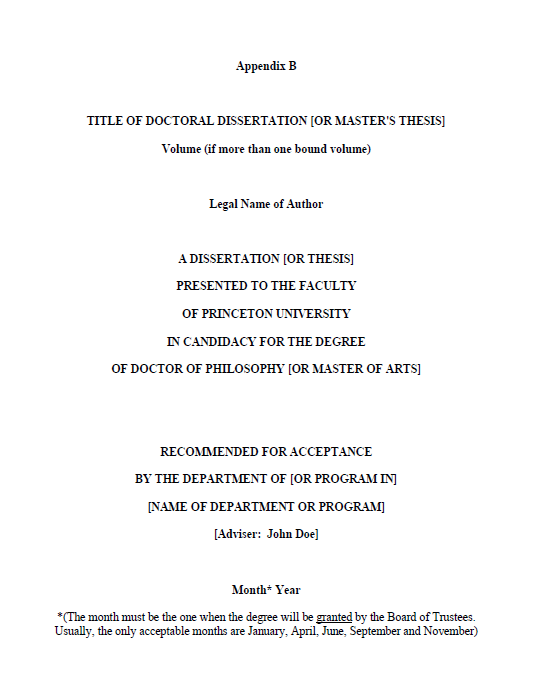
\includegraphics[width=0.9\linewidth]{ch-pastwork/figures/titlepage}
    \caption[Sample Title Page Layout]{Sample title page layout~\cite{muddthesis2009}}
    \label{fig:pastwork:titlepage}
  \end{center}
\end{figure}




\chapter{Usage\label{ch:usage}}

To start, in your main .tex file, use this class as your main documentclass instead of `report' or `book'. For example:
\begin{quote}
$\backslash documentclass[12pt,lot, lof]\{puthesis\}$
\end{quote}

In this example, we setup our document to use the PU Thesis style, with 12pt font for body text, and to include a List of Tables and List of Figures in the front matter. You could instead set an 11 point or 10 point font by changing the first option. You can also add `los' to include a list of symbols.

To use single spacing, add the option `singlespace'. This is a special option for the \texttt{puthesis} documentclass, which sets single spacing for both the front matter and for the document itself. Additional parameters should be set in your main .tex file, and are described in detail in Section~\ref{sec:usage:options}.

The template itself declares two other options, to be set immediately after the \texttt{documentclass} command. First is `printmode', declared with the command:
\begin{quote}
$\backslash newcommand\{\backslash printmode\}\{\}$
\end{quote}
This command, used later in the thesis.tex file, turns off the \texttt{hyperref} package and all internal links in the PDF file. This removes any colored links and highlighting that would not be appropriate in a printed and bound thesis. Instead the \texttt{url} package is loaded, so that \\url commands in your document will continue to work and urls will break properly across multiple lines.

When `printmode' is not specified, the hyperref package is included. It creates colored links for citations, footnotes, and internal references, which can be used to navigate the PDF document more easily. It also adds bookmarks to the PDF file, mirroring the table of contents. By default, it is set to use colored links. For the PDF file that you will submit electronically to ProQuest, this may not be desirable since some copies may be printed, while others will be used electronically. Thus another option, `proquestmode', is defined that keeps hyperref but disables colored links:
\begin{quote}
$\backslash newcommand\{\backslash proquestmode\}\{\}$
\end{quote}
This mode has no effect when used in combination with `printmode'. 


\section{Options}
\label{sec:usage:options}

In this section, we describe the options you can set when using this thesis class.
\tablespacing
% tablespacing is defined by the class to set single spacing for the long table when in doublespacing mode. If the singlespace option is set, this command has no effect.

\begin{longtable}{p{0.3\linewidth} p{0.6\linewidth}}

  % First page heading
  \caption[Options Provided by the PUthesis Class]{List of options for the puthesis document class and template} \label{tab:usage:options}\\
  \toprule
  \textbf{Option} & \textbf{Description} \\
  \midrule
  \endfirsthead

  % Future page heading
  \caption[]{(continued)}\\
  \toprule
  \textbf{Option} & \textbf{Description} \\
  \midrule
  \endhead

  % Page footer
  \midrule
  \multicolumn{2}{r}{(Continued on next page)}\\
  \endfoot

  % Last page footer
  \bottomrule
  \endlastfoot

  12pt &
  Specify the font size for body text as a parameter to \texttt{documentclass}. The Mudd Library requirements~\cite{muddthesis2009} state that 12pt is preferred for serif fonts (e.g., Times New Roman) and 10pt for sans-serif fonts (e.g., Arial).
  \\

  letterpaper &
  If your document is coming out in a4paper, your LaTeX defaults may be wrong. Set this option as a parameter to \texttt{documentclass} to have the correct 8.5"x11" paper size.
  \\

  lot &
  Set this option as a parameter to \texttt{documentclass} to insert a List of Tables after the Table of Contents.
  \\


  lof &
  Set this option as a parameter to \texttt{documentclass} to insert a List of Figures after the Table of Contents and the List of Figures.
  \\

  los &
  Set this option as a parameter to \texttt{documentclass} to insert a List of Symbols after the Table of Contents and the other lists.
  \\

  singlespace &
  Set this option as a parameter to \texttt{documentclass} to single space your document. Double spacing is the default otherwise, and is required for the electronic copy you submit to ProQuest. Single spacing is permitted for the printed and bound copies for Mudd Library.
  \\
  
  draft &
  Set this option as a parameter to \texttt{documentclass} to have \LaTeX mark sections of your document that have formatting errors (e.g., overfull hboxes). 
  \\

  % the cmidrule here spans both columns but is indented slightly on the left and right. 
  \cmidrule[0.1pt](l{0.5em}r{0.5em}){1-2}

  \raggedright
  $\backslash newcommand$ $\{\backslash printmode\}\{\}$ &
  Insert this command after the \texttt{documentclass} command to turn off the hyperref package to produce a PDF suitable for printing.
  \\

  \raggedright
  $\backslash newcommand$ $\{\backslash proquestmode\}\{\}$  &
  Insert this command after the \texttt{documentclass} command to turn off the `colorlinks' option to the hyperref package. Links in the pdf document will then be outlined in color instead of having the text itself be colored. This is more suitable when the PDF may be viewed online or printed by the reader.
  \\

  $\backslash makefrontmatter$ &
  Insert this command after the \texttt{$\backslash begin\{document\}$} command, but before including your chapters to insert the Table of Contents and other front matter.
  \\
  
  \cmidrule[0.1pt](l{0.5em}r{0.5em}){1-2}

  $\backslash title$ &
  Set the title of your dissertation. Used on the title page and in the PDF properties.
  \\

  $\backslash submitted$ &
  Set the submission date of your dissertation. Used on the title page. This should be the month and year when your degree will be conferred, generally only January, April, June, September, or November. Check the Mudd Library rules~\cite{mudd2009} for the appropriate deadlines.
  \\

  $\backslash copyrightyear$ &
  Set the submission year of your dissertation. Used on the copyright page.
  \\

  $\backslash author$ &
  Your full name. Used on the title page, copyright page, and the PDF properties. \\

  $\backslash adviser$ &
  Your adviser's full name. Used on the title page. \\

  $\backslash departmentprefix$ &
  The wording that precedes your department or program name. Used on the title page. The default is ``Department of'', since most people list their department and can leave this out (e.g., Department of Electrical Engineering), however if yours is a program, set $\backslash departmentprefix\{Program in\}$ \\

  $\backslash department$ &
  The name of your department or program. Used on the title page. \\

  \cmidrule[0.1pt](l{0.5em}r{0.5em}){1-2}
  
  \raggedright  
  $\backslash renewcommand$ $\{\backslash maketitlepage\}\{\}$ &
  Disable the insertion of the title page in the front matter. This is useful for early drafts of your dissertation. \\

  \raggedright  % full justification places the * in an awkward place
  $\backslash renewcommand*\{\backslash makecopyrightpage\}\{\}$ &
  Disable the insertion of the copyright page in the front matter. This is useful for early drafts of your dissertation. \\

  \raggedright 
  $\backslash renewcommand*\{\backslash makeabstract\}\{\}$ &
  Disable the insertion of the abstract in the front matter. This is useful for early drafts of your dissertation. \\

\end{longtable}
\bodyspacing
% bodyspacing restores double spacing or single spacing after the table

% need blank space after \bodyspacing

I've seen other people print their dissertations using $\backslash pagestyle\{headings\}$, which places running headings on the top of each page with the chapter number, chapter name, and page number. This documentclass is not currently compatible with this option -- the margins are setup to be correct with page numbers in the footer, placing them 3/4" from the edge of the paper, as required. If you wish to use headings, you will need to adjust the margins accordingly.
 




\chapter{Implementation Details\label{ch:implementation}}

Appendices are just chapters, included after the $\backslash appendix$ command.

\section{Switching Formats}
When switching \texttt{printmode} on and off (see Section~\ref{sec:usage:options}), you may need to delete the output .aux files to get the document code to compile correctly. This is because the hyperref package is switched off for \texttt{printmode}, but this package inserts extra tags into the contents lines in the auxiliary files for PDF links, and these can cause errors when the package is not used.

\section{Long Tables}

Long tables span multiple pages. By default they are treated like body text, but we want them to be single spaced all the time. The class therefore defines a new command, $\backslash tablespacing$, that is placed before a long table to switch to single spacing when the rest of the document is in double spacing mode. Another command, $\backslash bodyspacing$, is placed after the long table to switch back to double spacing. Normal tables using \texttt{tabular} automatically use single spacing and do not require the extra commands.

When the documentclass is defined with the `singlespace' option, these commands are automatically adjusted to stay in single spacing after the long table.

Make sure there is always at least one blank line after the $\backslash bodyspacing$ command before the end of the file.

Some times long tables do not format correctly on the first pass. If the column widths are wrong, try running the \LaTeX compiler one or two extra times to allow it to better calculate the column widths.

If you want your long table to break pages at a specific point, you can insert the command $\backslash pagebreak[4]$, to tell \LaTeX that it really should put a page break there. $\backslash pagebreak[2]$ gives it a hint that this is a good place for a page break, if needed. If there's a row that really should not be broken across a page, use $\backslash \backslash *$, which will usually prevent a pagebreak. 

\section{Booktabs}
The booktabs package is included to print nicer tables. See the package documentation~\cite{fear2005booktabs} for more details and motivation. Generally, all vertical lines are removed from the tables for a better visual appearance (so don't put them in), and better spacing and line thicknesses are used for the horizontal rules. The rules are defined as $\backslash toprule$ at the top of the table, $\backslash midrule$ in between the heading and the body of the table (or between sections of the table), and $\backslash bottomrule$ at the end of the table. $\backslash cmidrule$ can be used with the appropriate options to have a rule that spans only certain columns of the table.

\section{Bibliography and Footnotes}

The bibliography and any footnotes can also be single spaced, even for the electronic copy. The template is already setup to do this.

Bibliography entries go in the .bib file. As usual, be sure to compile the \LaTeX code, then run BibTeX, and then run \LaTeX again.

To cite websites and other electronically accessed materials, you can use the `@electronic' type of BibTeX entry, and use the `howpublished' field to include the URL of the source material.

The formatting of bibliography entries will be done automatically. Usually the titles are changed to have only the first word capitalized. If you'd prefer to have your original formatting preserved, place the title in an extra set of curly braces, i.e., ``title = \{\{My title has an AcroNyM that should stay unchanged\}\},''.

\section{Figures and Tables}
The captions of figures and tables take an optional parameter in square brackets, specifying the caption text to be used in the Table of Contents. The regular caption in curly braces is used for the table itself.

Generally captions for tables are placed above the table, while captions for figures are placed below the figure.




\chapter{Printing and Binding\label{ch:printing}}

\section{Printing}

For the library copies of your dissertation, you must use archival quality printing and binding. This means acid-free paper, containing at least 25\% cotton fiber. Triangle Repocenter on Nassau Street in Princeton offers both 25\% cotton paper and 100\% cotton paper. Most people choose the 25\% cotton paper, and this is generally recommended by the binders. The 100\% copy paper is somewhat thicker and the extra expense is unnecessary. 

Triangle offers online submission of your printing and binding order at: \url{http://triangleprinceton.com/collegiatebinding/thesis/}. If you request binding from them, they will deliver the paper copies to Smith-Shattuck Bookbinding for you and allow you to pick up the completed copies at their store on Nassau Street. The whole process takes 2-3 business days, but check with them in advance during the busy thesis-printing season in April and May. 

Currently, your printed and bound dissertation copies can be single spaced. Only the electronic copy submitted to ProQuest must be double spaced. All copies must be printed single-sided, with specific margins. 

\section{Binding}

An archival-quality sewn binding is required for the library copies of your dissertation. Smith-Shattuck Bookbinding is highly recommended, and is used by most students. Triangle Repocenter will send your copies there for you, greatly simplifying the process, but you can call Smith-Shattuck with special requests. 

The ``library standard'' sewn binding is sufficient for the copies to be sent to Mudd Library. It uses a black buckram cloth cover, which is the most popular option. For extra copies for yourself and your family members, you can choose ``buckram roundback binding'', which adds decorative lines on the spine, and printing of the title and author on the front cover. For a small additional fee, you can include the Princeton University shield on the front cover and a ribbon bookmark. Leather covers are also available. See Smith-Shattuck's website for more details at: \url{http://www.thesisbookbinding.com/}. 


% Make the bibliography single spaced
\singlespacing
% Switched to BibLatex instead
% \bibliographystyle{apacite}

% add the Bibliography to the Table of Contents
\cleardoublepage
\ifdefined\phantomsection
  \phantomsection  % makes hyperref recognize this section properly for pdf link
\else
\fi
\addcontentsline{toc}{chapter}{Bibliography}

% include your .bib file
\printbibliography

\end{document}

